\documentclass[twoside, 11pt]{report}
\usepackage[a4paper,width=150mm,top=25mm,bottom=25mm,bindingoffset=6mm, hcentering]{geometry}
\usepackage[czech]{babel}


% HEADER nastaveni
\usepackage{fancyhdr} 
\pagestyle{fancy}
\usepackage{fancyvrb}       % vylepšené prostředí pro strojové písmo
\fancyhead{}
% sections se objevuji vlevo nahore, pokud je
%\fancyhead[RE,LO]{\rightmark}
% Chapters se objevuji vpravo nahore
\fancyhead[LE]{\chaptername~\thechapter}
\fancyhead[LE]{\leftmark}
\fancyhead[RO]{\rightmark}
\usepackage{amsfonts,amssymb}
\usepackage{amsmath}
\usepackage[none]{hyphenat}
\usepackage{graphicx}
\usepackage{float}
\usepackage{color}
\usepackage{epsfig}
\usepackage{xcolor}
\usepackage{hyperref}
\usepackage{xcolor}
\hypersetup{
	colorlinks,
	linkcolor={blue!50!black},
	citecolor={blue!50!black},
	urlcolor={blue!80!black}
}
\usepackage{multirow}
\usepackage{subcaption}
\usepackage{caption}
\usepackage{svg}
\usepackage{subcaption}
\usepackage{transparent}
\usepackage{epsfig}
\usepackage{epstopdf}
\usepackage{physics}
\usepackage{mathtools}
\usepackage{mhchem}
\usepackage{graphicx}
\usepackage{pdfpages}
\usepackage{lipsum}
\usepackage[toc,page]{appendix}
\usepackage[toc]{glossaries}
\graphicspath{ {./ObrazkyDP/} }
\usepackage{notoccite}

% for insert some CODE
\usepackage{listings}
\definecolor{mygreen}{rgb}{0,0.6,0}
\definecolor{mygray}{rgb}{0.5,0.5,0.5}
\definecolor{mymauve}{rgb}{0.58,0,0.82}
\lstset{ %
	backgroundcolor=\color{white},   % choose the background color
	basicstyle=\footnotesize\ttfamily,        % size of fonts used for the code
	breaklines=true,                 % automatic line breaking only at whitespace
	captionpos=b,                    % sets the caption-position to bottom
	commentstyle=\color{mygreen},    % comment style
	escapeinside={\%*}{*)},          % if you want to add LaTeX within your code
	keywordstyle=\color{blue},       % keyword style
	stringstyle=\color{mymauve},     % string literal style
}
\renewcommand{\lstlistingname}{Kód}


\usepackage{afterpage}
\newcommand\blankpage{%
	\null
	\thispagestyle{empty}%
	%\addtocounter{page}{-1}%
	\cleardoublepage}

\usepackage{array}
\newcolumntype{P}[1]{>{\centering\arraybackslash}p{#1}}

\renewcommand{\figurename}{Obr.}
\newcommand\myeq{\stackrel{\mathclap{\normalfont\mbox{?}}}{=}}



% Typograficke konvence
\usepackage[all]{nowidow}
\pretolerance=5000
\tolerance=9000
\emergencystretch=0pt
\righthyphenmin=4
\lefthyphenmin=4
\linespread{1.3}

% Toto makro definuje kapitolu, která není očíslovaná, ale je uvedena v obsahu.
\def\chapwithtoc#1{
	\chapter*{#1}
	\addcontentsline{toc}{chapter}{#1}
}

%%% Prostředí pro sazbu kódu, případně vstupu/výstupu počítačových
%%% programů. (Vyžaduje balíček fancyvrb -- fancy verbatim.)
\DefineVerbatimEnvironment{code}{Verbatim}{fontsize=\small, frame=single}

\begin{document}
	\begin{titlepage}
		\begin{large}
			\begin{flushleft}
				\textsc{České vysoké učení technické v Praze}\\
				\textsc{Fakulta Elektrotechnická}\\
				\textsc{Katedra Mikroelektroniky}\\
			\end{flushleft}
		\end{large}
		\begin{center}
			\vspace{1.5 cm}
			
\includegraphics[width=7cm]{symbol.jpg}\\[1.0 cm]
			{Diplomová práce}\\[0.5 cm]
			\vspace{1.5 cm}
			{\Large Miniaturizované vyčítací rozhraní pro pixelový detektor radiace Timepix 2} \\[1.5cm]
			{\textit {Ondřej Pavlas}}\\[1.0 cm]
			{Vedoucí: Ing. Záhlava Vít, CSc.}\\[1.0 cm]
			Studijní program: Elektronika a komunikace\\
			{Květen 2024}
		\end{center}
	\end{titlepage}
	
% prázdná stránka
\thispagestyle{empty}
\afterpage{\blankpage}
\clearpage

	
%\setcounter{page}{1}
\pagenumbering{roman}
\setcounter{page}{3}

% Declaration
\chapter*{Prohlášení:}
Prohlašuji, že jsem předloženou práci vypracoval samostatně a že jsem uvedl veškeré použité informační zdroje v souladu s Metodickým pokynem o dodržování etických principů při přípravě vysokoškolských závěrečných prací.\newline


\noindent Praha, dne ........................ \hfill ..........................................
\noindent \begin{flushright}
podpis
\end{flushright}


\chapter*{Poděkování:}
TODO poděkování

% Abstract
\newpage
\thispagestyle{plain}

\begin{center}
	\Large
	\textbf{Abstract}
\end{center}

TODO English abstract


%\textbf{Keywords:} keyword.

\hfill

\begin{center}
	\Large
	\textbf{Abstrakt}
\end{center}

TODO Český abstrakt

%obsah
\newgeometry{margin=2cm,top=2cm}
\thispagestyle{empty}
\tableofcontents


%seznam obrazku
\listoffigures
\newpage
\listoftables
\newpage
\restoregeometry

\pagenumbering{arabic}


%TEXT PRACE
% input CHAPTER

% TODO rozmyslet kam dat obrazek finalniho zarizeni: Abstrakt, Uvod ?

% Úvod
\chapter{Úvod}

% + žvásty o používání pixelových detekrorů -> nahnat reference

%TODO zminit UTEF, tady nebo v abstraktu?

Cílem této diplomové práce je realizace miniaturizovaného vyčítacího rozhraní pro pixelový detektor radiace Timepix 2. Realizace diplomové práce probíhala na půdě Ústavu Technické a Experimentální Fyziky ČVUT v Praze. Diplomová práce je rozčleněna do následujících čtyř hlavních částí.

\par \hyperref[kap:2]{První část} práce se týká pixelových detektorů radiace a vyčítacích zařízení. V této kapitole bude popsán obecný princip činnosti pixelových detektorů, především generace detektorů z rodiny Timepix, vyvíjených pod záštitou CERN Medipix Collaboration \cite{Medpix}. Dále zde bude uvedeny příklady vyčítacích rozhraní, která jsou nezbytnou součástí pro vyčítaní dat z detektorů Timepix.

\par \hyperref[Koncept reseni]{Druhá část} obsahuje koncept návrhu řešení této diplomové práce. V této části bude diskutováno, jaké parametry vyčítací rozhraní musí splňovat, aby byla zajištěna základní funkcionalita navrženého rozhraní.

\par \hyperref[realizace]{Třetí část} textu obsahuje podrobný popis realizace miniaturizovaného vyčítacího rozhraní pro pixelový detektor Timepix 2. Podkapitoly této části jsou rozděleny do logických bloků, jež odpovídají samotným blokům skutečné realizace. Bude zde podrobně popsáno schematické zapojení a parametry navrženého rozhraní.

\par \hyperref[testovani]{Čtvrtá část} je tvořena funkčními testy navrženého rozhraní a ověřením funkcionality rozhraní jako celku. Je zde popsáno testování jednotlivých funkčních celků, tak celého rozhraní. Komplexním testem pro navržené vyčítací rozhraní je poté připojení rozhraní do programu TrackLab \cite{Manek_2024} a obsluha rozhraní za využití právě tohoto programu. Finálním funkčním testem popsaným v této části je samotné měření s navrženým miniaturizovaným vyčítacím rozhraní, které bylo realizováno v laboratoři CERN.

\chapter{Pixelové detektory radiace a vyčítací zařízení}	% + pro pixelové detektory
\label{kap:2}
Mezi možnosti detekovat ionizující záření patří mimo jiné, použití pixelových detektorů. Pomocí pixelových detektorů, konkrétněji hybridních pixelových detektorů, jsme schopni detailně změřit ionizující záření. V dalších částech této kapitoly bude popsána obecná činnost a princip detekce radiace pixelových detektorů. V části \ref{Timepix2}, bude konkrétně popsán detektor z rodiny Timepix \cite{Llopart}, detektor Timepix 2 \cite{tpx2_manual}. 

\section{Princip činnosti pixelových detektorů}
\label{kap:2.1}
V této části bude popsán obecný princip činnosti pixelových detektorů, který je společný pro detektory radiace z rodiny Timepix \cite{Llopart}, vyvíjenými pod záštitou CERN Medpipix Collaboration \cite{Medpix}. Pixelový detektor, přesněji hybridní pixelový detektor se skládá ze dvou oddělitelných částí, ze senzorové vrstvy a vrstvy s vyčítací elektronikou viz. obrázek \ref{fig:Timepix}. Právě toto rozdělení na senzorovou a vyčítací část označuje název hybridní detektor.
\par Senzorová vrstva je tvořena polovodičovým materiálem. Důležitými parametry senzorové vrstvy jsou typ polovodičového materiálu a její tloušťka. Nejčastěji používané materiály jsou $\text{Si}$, $\text{CdTe}$ a $\text{GaAs}$. Na senzorovou vrstvu je připojené vysoké napětí, označované jako \textit{bias voltage}. Toto vysoké napětí zajistí vyprázdnění oblasti v polovodičové struktuře senzorové vrstvy. Pokud částice ionizujícího záření interaguje v senzorové vrstvě, dojde k vytvoření náboje. Tento náboj je dále zpracován vyčítací elektronikou která je pomocí technologie nazývající se \textit{bump bond}, připojena k senzorové vrstvě.
\par Vyčítací vrstva (ASIC) je rozdělena na 256x256 individuálních pixelů. Každý pixel obsahuje potřebnou elektroniku ke zpracovaní náboje, vzniklého v senzorové vrstvě. Detailnější popis zpracování analogového náboje na úrovni jednotlivých pixelů, bude popsán pro konkrétní pixelový detektor Timepix 2 v části \ref{Timepix2}. Po analogovém zpracování signálu následuje digitální zpracování, poté je digitální signál převeden na výstupní plošky. Vyčítací vrstva je pomocí \textit{wire bond} technologie připojena k desce plošných spojů. Signály vedoucí z pixelových detektorů jsou následně zpracovány vyčítacím zařízením. Druhy vyčítacích zařízní budou popsány v části \ref{Vycitaci zarizeni}.
 \begin{figure}[h!]
 	\centering
 	\captionsetup{justification=centering}
 	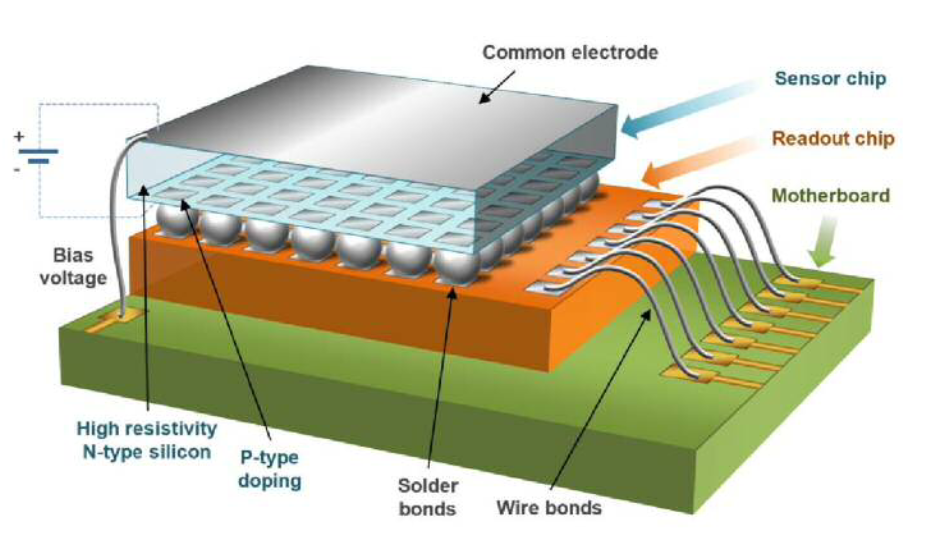
\includegraphics[scale=0.55]{Timepix.png}
 	\caption{Rozložení hybridního pixelového detektoru Timepix \cite{Platkevic}} 
 	\label{fig:Timepix}
 \end{figure}	

\section{Vyčítací zařízení pro pixelové detektory}
\label{Vycitaci zarizeni}
Každý pixelový detektor z rodiny detektorů Timepix \cite{Llopart}, má specifické požadavky pro návrh vyčítacího zařízení. Základními požadavky jakými jsou napájecí napětí detektoru a komunikační rozhraní s detektorem, musí být vždy splněny aby bylo možné spolehlivě komunikovat s pixelovým detektorem. Vyčítacích zařízení existuje celá řada. V této práci, respektive v následujících částech bude popsán návrh miniaturizovaného vyčítacího rozhraní. Pokusím se zde tedy uvést příklady miniaturizovaných zařízení.
\subsection{USB Lite}
Dosud nejmenším vyčítacím zařízení rodiny detektorů Timepix \cite{Llopart}, je zařízení \textit{USB Lite} \cite{usb_lite}, viz. obrázek \ref{fig:usb_lite}. Toto zařízení umožňuje komunikovat s detektorem Medipix 2 \cite{Medpix2}. Rozměry zařízení jsou 60x15 mm. Rychlost vyčítání snímků je 4 fps a spotřeba zařízení je menší než 2 W \cite{usb_lite}.
 \begin{figure}[h!]
	\centering
	\captionsetup{justification=centering}
	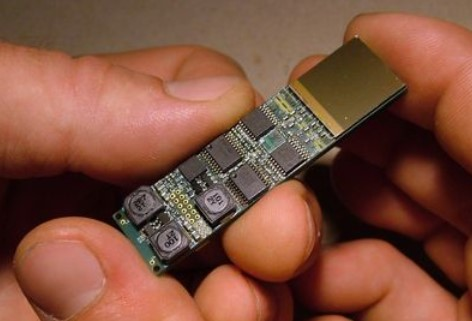
\includegraphics[scale=0.55]{usb_lite.jpg}
	\caption{Vyčítací zařízení \textit{USB lite}} 
	\label{fig:usb_lite}
\end{figure}	

\subsection{MiniPIX SPRINTER}
Vyčítací zařízení MiniPIX SPRINTER je vyvíjeno společností ADVACAM, zařízení je možné vidět na obrázku \ref{fig:sprinter}. Toto zařízení umožňuje komunikovat s detektorem Timepix 2 \cite{tpx2_manual}. Rozměry zařízení jsou 50x21x14 mm. Rychlost vyčítání snímků je 99 \cite{Advacam}.
\begin{figure}[h!]
	\centering
	\captionsetup{justification=centering}
	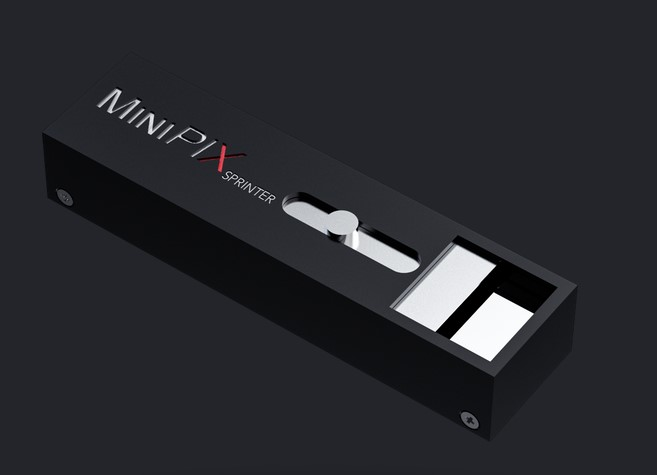
\includegraphics[scale=0.55]{sprinter.jpg}
	\caption{Vyčítací zařízení MiniPIX SPRINTER} 
	\label{fig:sprinter}
\end{figure}	

\subsection{Katherine pro Timepix 2} %katherine zminena protoze modularita
Posledním uvedeným tipem vyčítacího zařízení je zařízení Kathrine pro Timepix 2, které můžete vidět na obrázku \ref{fig:Katherine2}. Toto vyčítací zařízní se od předchozích dvou uvedených liší ve velikosti a maximalní rychlosti komunikace. Zařízení se skládá ze dvou částí. Samotným vyčítacím zařízením, na obrázku \ref{fig:Katherine2} vpravo a takzvaným \textit{chipboardem}, na obrázku \ref{fig:Katherine2} vlevo. Část chipboardu obsahuje detektor Timepix 2 a napájecí zdroje potřebné pro provoz detektoru. Dále jsou ze propojeny signály z konektoru od vyčítacího zařízení po samotný Timepix 2. Výhodou tohoto modulárního zapojení je možnost modifikace chipboardové části, bez nutnosti změn na straně vyčítacího zařízení. Tedy existuje možnost k jednomu vyčítacímu zařízení, připojit různé chipboardy. Parametry samotného vyčítacího zařízení jsou následující. Rozměry 100x80x28 mm, rychlost vyčítaní až 3.2 Gbps \cite{Burian_2020}.
\begin{figure}[h!]
	\centering
	\captionsetup{justification=centering}
	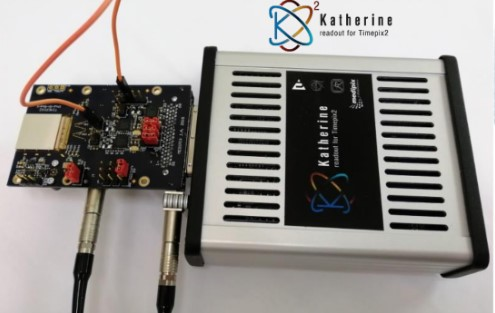
\includegraphics[scale=0.75]{Katherine2.jpg}
	\caption{Vyčítací zařízení Katherine pro Timepix 2 \cite{Burian_2020}} 
	\label{fig:Katherine2}
\end{figure}	

%%%
%%%%%%%%%%%%%%%%%%%%%%%%%%%

\section{Timepix 2}
% v podstatě technická dokumentace Timepix 2, plus konkretni pozadavky pro provoz
\label{Timepix2}
V předchozí části \ref{kap:2.1}, byly popsány obecné vlastnosti detektoru a základní principy detekce ionizujícího záření. V této kapitole bude detailněji popsán konkrétní detektor, detektor Timepix 2 \cite{tpx2_manual}. Detektor byl vyvinut pod záštitou CERN Medpipix Collaboration \cite{Medpix}. Timepix 2 patří do rodiny detektorů Timepix. Prvním z rodiny detektorů byl detektor Timepix \cite{Llopart}, následně to popořadě byly detektory Timepix 3 \cite{Timepix3}, Timepix 2 \cite{tpx2_manual}, \cite{Timepix2} a nejnovějším detektorem je Timepix 4 \cite{Timepix4}. Detektor Timepix 2 je zobrazen na obrázku \ref{fig:Timepix2}.
\begin{figure}[h!]
	\centering
	\captionsetup{justification=centering}
	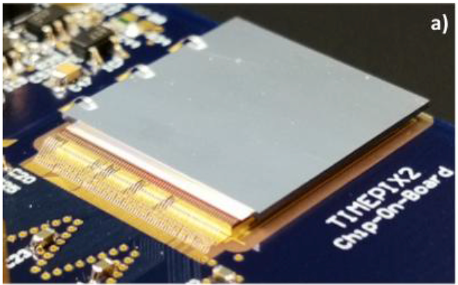
\includegraphics[scale=0.80]{Timepix2.png}
	\caption{Detektor Timepix 2 \cite{Timepix2}} 
	\label{fig:Timepix2}
\end{figure}	

\subsection{Analogová část}	 %todo upravit
Každý pixel z matice 256x256 pixelů má vlastní analogovou částí. Jak bylo zmíněno v kapitole \ref{kap:2}, pokud částice interaguje na senzorové vrstvě dojde k vytvoření nábojového impulsu. Tento náboj je díky připojenému napětí přitažen k elektrodám. Tento náboj může být charakterizován jako Diracův proudový impuls. Integrací Diracovo proudového impulsu dostaneme celkový generovaný náboj Q. Diracův impuls je naintegrován do malého kapacitoru Cf. Poté na výstupu CSA je v ideálním případě napěťový skok s amplitudou Q/Cf viz. \ref{fig:pixel_frontend}. Výstupní puls je poté porovnán s prahovou úrovní. Nastavením prahové úrovně lze eliminovat zbytkový proud, takzvaný \textit{leakage current}, závěrného směru polovodičové struktury, který zde vznikl kvůli připojenému vysokému napětí. Pokud je signál větší než daná nastavená úroveň, je inkrementován digitální čítač \cite{Llopart}. Každý diskriminátor obsahuje 5-bitový DAC převodník. Tento 5 bitový DAC převodník umožňuje nastavit úroveň detekovatelného signálu pro každý pixel individuálně a tím eliminovat šum. Uuspořádaní pro analogovou část lze vidět na obrázku \ref{fig:tpx2_cel}, kde je zobrazeno uspořádání jednoho pixelu detektoru Medipix 2.
\begin{figure}[h!]
	\begin{subfigure}{0.5\textwidth}
	\centering
	\captionsetup{justification=centering}
	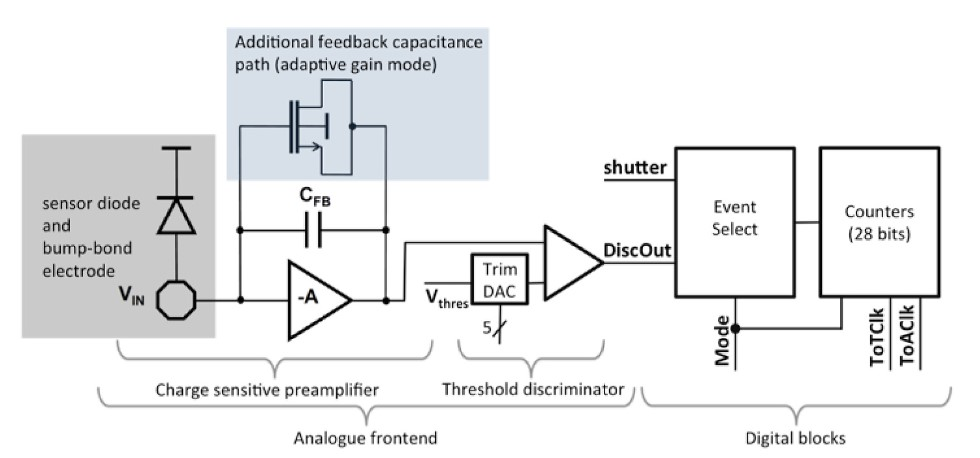
\includegraphics[scale=0.70]{tpx2_cel.jpg}
	\caption{Uspořádání jednoho pixelu} 
	\label{fig:tpx2_cel}
	\end{subfigure}
	\begin{subfigure}{0.5\textwidth}
		\centering
		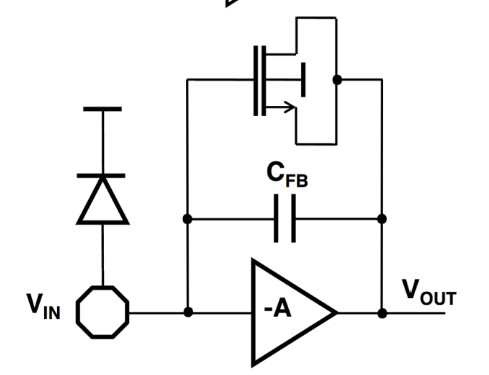
\includegraphics[scale=0.50]{pixel_frontend.jpg}
		\caption{První stupeň zpracování signálu, CSA}
		\label{fig:pixel_frontend}
	\end{subfigure}
	\caption{Zpracování signálu na úrovni pixelů}
	\label{fig:zpracování signálu}
\end{figure}

\subsection{Digitální část}
\label{Digitálni cast}
Každý pixel obsahuje čtyři digitální čítače typu LSFR. Každý n-bitový čítač generuje $2^n$ pseoudonáhodných čísel. V případě Timepix 2 každý pixel obsahuje dva 10-bitové (A,B) a dva 4-bitové (C,D) čítače. Například tedy 14-bitový čítač vznikne kombinací 10-bitového a 4-bitového čítače. Odpovídající 14-bitová hodnota je poté viz \ref{eq:1}. Celkem tedy pro každý pixel lze využít 28-bitů. Tyto čítače mouhou pracovat v různých módech. Tyto módy budou probrány v další části.
\begin{equation}
	14-bit = (hodnota_{4-bit} \cross 2^{10}) + hodnota_{10-bit}
	\label{eq:1}
\end{equation}

Jak bylo zmíněno výše. Každý z digitálních čítačů může být nakonfigurován do jiného módu. Pro Timepix 2 jsou to následující módy \ref{fig:modes}. 
\begin{itemize}
	\item \textbf{Time over Threshold} (ToT): Čítač je inkrementován při každým hodinovým pulsu, kdy je signál nad nastavenou prahovou úrovní
	\item \textbf{Time of Arrival} (ToA): Čítač je inkrementován při každým hodinovým pulsu, kdy signál překročí nastavenou úroveň a inkrementuje se až do konce akvizice.
	\item \textbf{Coutnig mode}: Čítač je inkrementován pokud signál překročí dvakrát nastavený práh, viz. obrázek \ref{fig:modes} 
\end{itemize}
\begin{figure}[h!]
	\centering
	\captionsetup{justification=centering}
	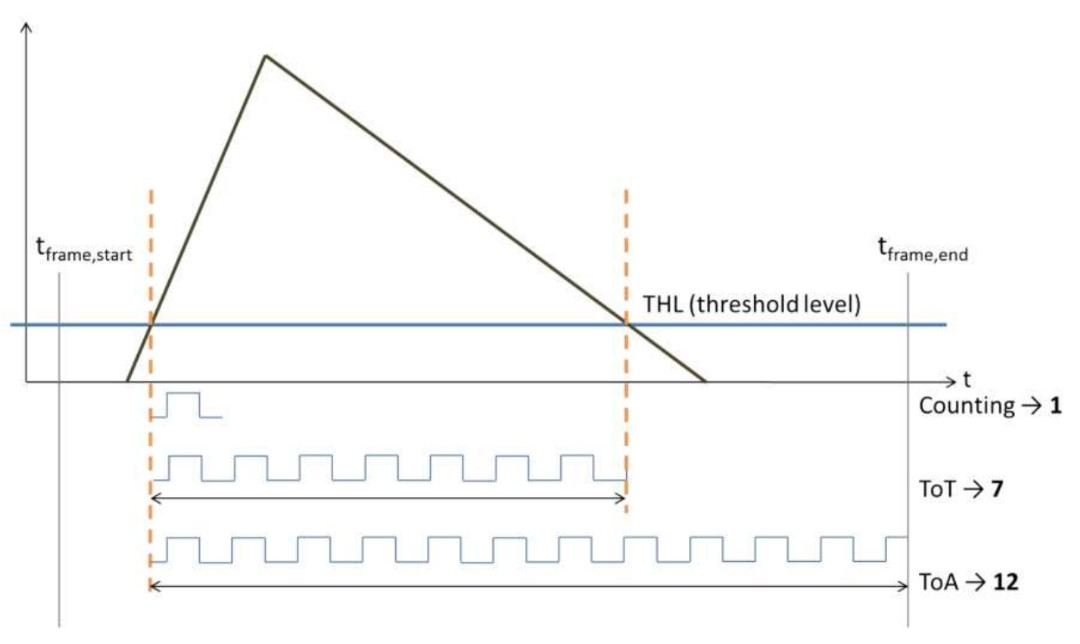
\includegraphics[scale=0.45]{modes.jpg}
	\caption{Digitální módy Timepix 2 \cite{Manek}} 
	\label{fig:modes}
\end{figure}	

Jakou energii interagující částice zanechala v senzoru můžeme zjistit z ToT měření. Počet hodinových cyklů odpovídá času, po který hodnota analogového napětí byla nad nastavenou detekovatelnou úrovní. Více o způsobu měření energie například viz. \cite{JAKUBEK2011S262}.

%TODO zminit ze countery mouhu ruzne kombinovat a zaroven jejich mody. PLUS zminit maskovani pixelu -> spotreba

\subsection{Komunikační rozhraní}
\label{Komunikacni rozhrani}
\subsubsection{Logické úrovně} 	% TODO nazev
\label{kap:3.2.1}
Timepix 2 umožňuje komunikaci po paraelním nebo sériovém datovém kanálu. Pro komunikaci přes paraelní bránu je možno využít 32 paraelních vodičů. Paraelní brána dosahuje násobně vyšších přenosových rychlostí, než sériový kanál, viz. obrázek \ref{fig:rychlosti}. Dosažením takovýchto rychlostí je zapotřebí na straně vyčítací elektroniky použít velmi rychlé rozhraní, například FPGA.  
\par Veškerá sériová komunikace probíhá po diferenciálních datových párech. Konkrétně se jedná o specifikaci SLVS \cite{SLVS}. Napěťové úrovně této specifikace lze najít na obrázku \ref{fig:SLVS_LVDS}. Jak lze na obrázku \ref{fig:SLVS_LVDS} vidět, specifikace SLVS je analogická se specifikací LVDS \cite{LVDS}. Výhody sériové komunikace jsou především v návrhu a spotřebě vyčítacího zařízení. Maximální datové rychlost, respektive rychlost komunikačních hodin je dle \cite{tpx2_manual} 100 Mhz. Lze tedy pro návrh použít například mikroprocesor. Hlavní nevýhodou sériové komunikace je oproti paraelní komunikaci vyčítací rychlost, která je násobně nižší \ref{fig:rychlosti}.
\begin{figure}[h!]
	\centering
	\captionsetup{justification=centering}
	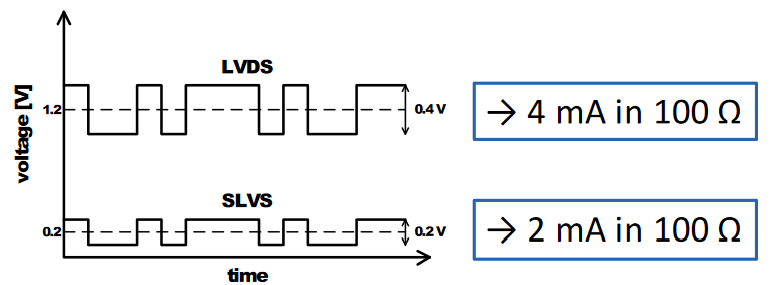
\includegraphics[scale=0.55]{SLVS_LVDS.png}
	\caption{SLVS specifikace \cite{SLVS}} 
	\label{fig:SLVS_LVDS}
\end{figure}	
\begin{figure}[h!]
	\centering
	\captionsetup{justification=centering}
	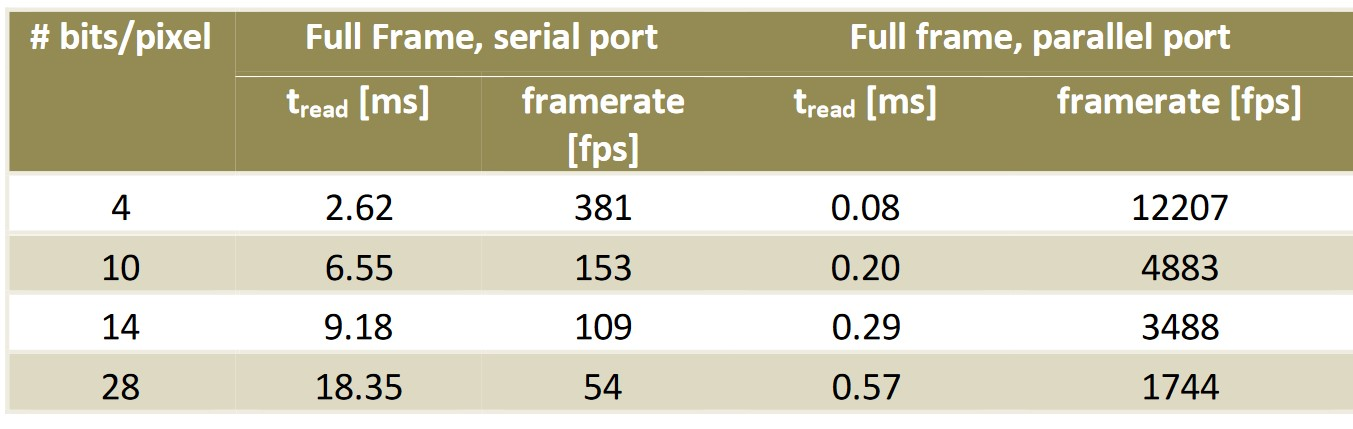
\includegraphics[scale=0.40]{rychlosti.jpg}
	\caption{Vyčítací rychlosti snímků z Timepix2. Frekvence hodin $f_{clock}$ = 100 MHz \cite{tpx2_manual}} 
	\label{fig:rychlosti}
\end{figure}	

\subsubsection{Struktura komunikace}
V této podkapitole bude popsána struktura komunikace s Timepix 2 za použití sériové komunikace popsané v \ref{kap:3.2.1}.  
%TODO popis signalu SPI pro TPX2 a casovani. Zminit i pakety SET/GET a jejich strukturu? 
Komunikace s Timepix 2 se rozděluje na příkazy SET a GET. Příkazy SET nastavujeme příslušný registr a příkazy GET daný registr vyčítáme. 
%TODO signaly potrebne pro komunikaci, ale pak i dac out atd ?.. 

%TODO MCLOCK
\subsection{Technická specifikace} %napáječky, kom. rozhraní, prikazy atd.., VN, hodiny pro měření, I/O piny
\label{Technicka specifikace}
Timepix 2 je rozdělen do 256 x 256 pixelů. Rozteč mezi jednotlivými pixely je 55 $\mu$$m$. Celkově pak Timepix 2 má rozměry 16.6 x 14.14 mm. Vyčítací část detektoru tvoří ASCI chip navržen ve 130 nm CMOS technologii. Samotná výroba ASIC je zajišťována jedním z předních výrobců chipů, firmou TSMC \cite{TSMC} na Taiwanu. Všechny technické informace, nebude-li uvedeno jinak jsou čerpány z manuálu k detektoru Timepix 2 \cite{tpx2_manual}.

\subsubsection{Napájení}	
Timepix 2 ke své činnosti potřebuj celkem 3 napájení viz. tabulka \ref{tab:tpx2_napajeni}. Napájení VDD a VDDA slouží k napájení jádra Timepix 2, napájení VDDIO pak k napájení vstupních výstupních bran. Pokud chceme z Timepix 2 vyčíst CHIP ID, musíme na pin VDD33 aplikovat napájecí napětí 2.5 V. Při normální činnosti detektoru, je požadováno napětí 1.2 V. Celková spotřeba Timepix 2 při zapnutí všech pixelů a frekvenci datových hodin $f_{clock}$ = Mhz je dle \cite{Timepix2} nižší než 900 mW.
\begin{table}[h!]
	\centering
	\begin{tabular}{ |P{3cm}||P{5cm}|  }
		\hline
		\multicolumn{2}{|c|}{Napájecí úrovně Timepix 2} \\
		\hline
		Název pinu& Hodnota napájecího napětí [V] \\ \hline \hline 
		VDDIO & 2.5 \\ \hline		
		VDD & 1.2 \\ \hline 		 
		VDDA & 1.2 \\ \hline
		VDD33 & 2.5 (1.2)\\ \hline
	\end{tabular}
	\caption{Napájecí úrovně Timepix 2}
	\label{tab:tpx2_napajeni}
\end{table}
%TODO HV
\par Speciální kategorií napájení je napájení pro zajištění vysokého napětí, které se připojí na senzorovou vrstvu. Toto napětí zajistí vyprázdnění oblasti v polovodičové struktuře. Požadavky na parametry vysokého napětí záleží na typu a tloušťce senzorové vrstvy. Nejčastěji používaným materiálem senzorové vrstvy je křemík. Příklad vysokého napětí, které bylo použito pro testování Timepix 2 se senzorovou vrstvou křemíku o tloušťce 500 $\mu$m dle \cite{Timepix2_500um} bylo 100 V. Další příklady velikosti vysokého napětí používaných pro různé senzorové vrstvy lze najít v odkazech \cite{Timepix_500um_Pospisil}, \cite{Timepix_500um_Huston}. Důležitou vlastností vysokonapěťových zdrojů je možnost nastavení výstupního vysokého napětí v určitém rozsahu.   

\subsubsection{Rozhraní pro připojení Timepix 2 k desce plošných spojů}	% TODO nazev
Připojení Timepix 2 k desce plošných spojů je nejčastěji realizováno pomocí technologie \textit{wire bonding}. Timepix 2 má celkem 152 pinů pro přichycení wire bondů. Rozložení pinů je zobrazeno na obrázku \ref{fig:tpx2_floorplan} ve spodní části. Rozteč mezi jednotlivými plošky je 108 $\mu$m.
\begin{figure}[h!]
	\centering
	\captionsetup{justification=centering}
	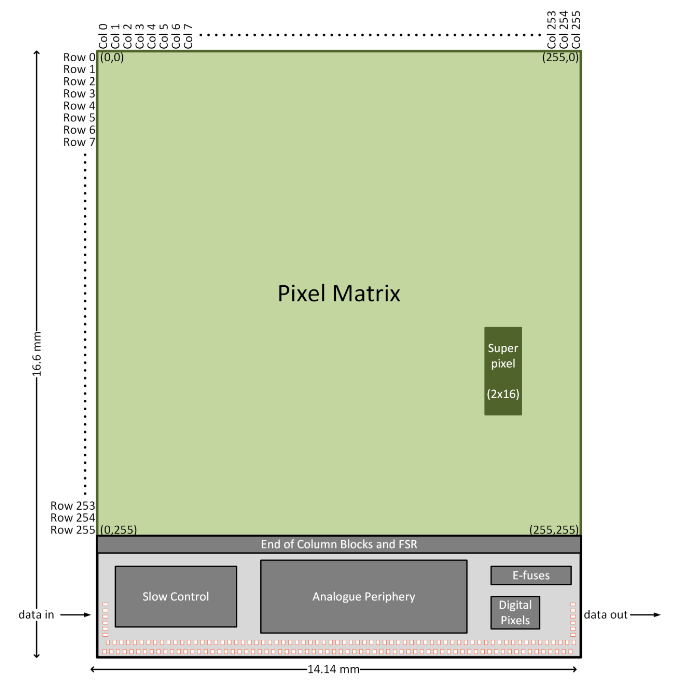
\includegraphics[scale=0.80]{tpx2_floorplan.png}
	\caption{Rozložení detektoru Timepix 2 \cite{tpx2_manual}} 
	\label{fig:tpx2_floorplan}
\end{figure}	
Dalším možným způsobem připojení Timepix 2 k desce plošných spojů je pomocí technologie zvané TSV. Respektive pomocí této technologie je možné signály vyvést ze zadní strany Timepix 2 k pájecím ploškám. Vznikne tím tak uspořádání, známe z technologie výroby pouzder BGA elektronických součástek. 
\par Běžnější způsob připojení Timepix 2 k desce plošných spojů je pomocí wire bondů. Použití wire bondů i technologie BGA je možné vidět na obrázku \ref{fig:bga}. Výhodou oproti technologii wire bondů je lepší praktické zacházení, díky absenci tenkých wire bondů, které jsou velmi náchylné na mechanické poškození. Další výhodou je poté technologicky méně náročné připojení detektoru. Avšak nevýhodou této technologie je vystavení chipu vysoké teplotě při pájení.
\begin{figure}[h!]
	\centering
	\captionsetup{justification=centering}
	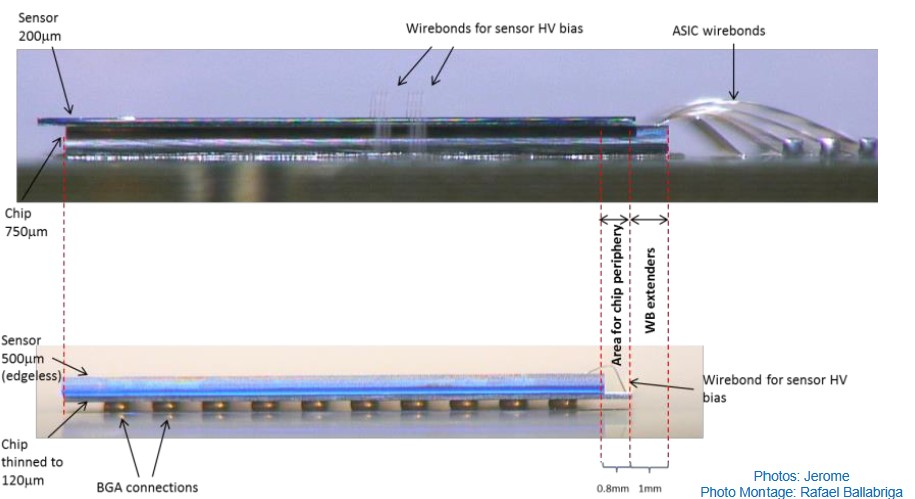
\includegraphics[scale=0.55]{bga.jpg}
	\caption{Připojení detektoru Timepix 2 k desce plošných spojů \cite{TSV}} 
	\label{fig:bga}
\end{figure}	











\chapter{Návrh řešení} % TODO lepe promyslet jak se ujmout teto casti
\label{Koncept reseni}
%popis jednotlivych bloku realizace, s odkazem na blokove schema z Kapitoly 3
Řešení bylo navrženo s ohled na primární požadavky, které rozhraní musí splňovat, aby byla zajištěna jeho základní funkčnost. Prvním primárním požadavkem, je zajištění základní funkčnosti detektoru Timepix 2, tyto požadavky byly popsány v části \ref{Technicka specifikace}. Dalším požadavkem na navrhované vyčítací rozhraní je jeho celková miniaturizace, tento požadavek byl stanoven zadním diplomové práce.
\par Podrobnější rozbor celkového řešení této práce, je dále v části \ref{realizace}, kde bude popsán výběr konkrétních součástek a návrh zapojení rozhraní, respektující primární požadavky uvedené v této části textu \ref{Koncept reseni}.

\section{Koncept řešení}
Navržený koncept vyčítacího rozhraní je zobrazen pomocí schematického nákresu na obrázku \ref{fig:navrh_reseni}. Koncept rozhraní se skládá ze dvou desek plošných spojů. 
\par První deskou plošných spojů je \textit{Základní deska} \ref{fig:navrh_reseni}. Na této desce je implementováno většina funkcionalit potřebných pro komunikaci s detektorem Timepix 2. Dále je zde implementována část zajišťující USB komunikaci, která slouží pro komunikaci s u uživatelským rozhraní přes USB.
\par Druhou deskou plošných spojů je \textit{Deska s Timepix 2} \ref{fig:navrh_reseni}. Na této desce se nachází detektor Timepix 2, dále je zde implementován vysokonapěťový zdroj (HV), měření vysokého napětí a teploty.
\par Toto rozložení rozhraní na dvě desky plošných spojů, bylo navrhnutu s ohledem na požadavky miniaturizace celého zařízení, a také s ohledem na variabilitu zařízení. Variabilitu myšlenou ve smyslu možnosti připojit k jedné základní desce různé desky s pixelovým detektorem, tento koncept lze také najít například v zařízení popsaném v části \ref{Katherine}. Koncept byl dále navrhnut s ohledem na možnost vyčítací rozhraní připojit k uživatelskému rozhraní, konkrétně k osobnímu počítači.  
\begin{figure}[h!]
	\centering
	\captionsetup{justification=centering}
	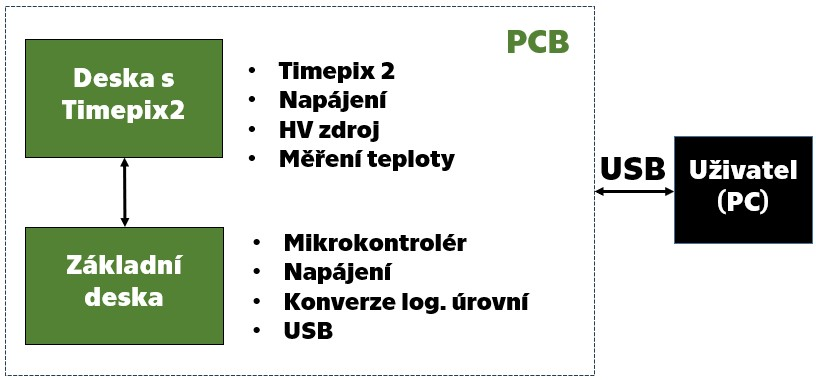
\includegraphics[scale=0.80]{navrh_reseni.jpg}
	\caption{Koncept řešení vyčítacího rozhraní pro detektor Timepix 2} 
	\label{fig:navrh_reseni}
\end{figure}

\subsection{Komunikace s Timepix 2}
Pro komunikaci s Timepix 2 je možné využít sériové, nebo paralelní rozhraní, jak již bylo zmíněno v části \ref{Komunikacni rozhrani}. Pro tuto práci uvažujme využití pouze sériové komunikace. Využití sériového rozhraní pro komunikaci s Timepix 2, umožní použít mikrokontrolér. Maximální vyčítací rychlost z detektoru Timepix 2 je 100 Mbits/s. S ohledem na tuto maximální rychlost vyčítaní dat z Timepix 2 musí být vybrán vhodný mikrokontrolér pro obsluhu komunikace, nejen s Timepix 2 detektorem. 

\subsection{Uživatelské komunikační rozhraní}
Komunikační rozhraní pro tuto práci bylo zvoleno rozhraní USB s konektorem typu C. Použit byl standart USB 2.0 High Speed. Tento standart umožňuje komunikovat maximální rychlostí až 480 Mbit/s. S respektem na maximální rychlost vyčítání dat z detektoru Timepix 2, která je 100 Mbits/s, je tato rychlost dostačující. 

\subsection{Napájení}
Pro napájení detektoru Timepix 2 jsou dle \ref{tab:tpx2_napajeni} zapotřebí tři napájecí napětí. Napájecí zdroje musí být vhodné pro maximální odběr detektoru Timepix 2. Kde uvedená celková spotřeba samotného detektoru, by neměla být dle \ref{Timepix2} vyšší než něž 900 mW. 
\par Dalším potřebným napájením potřebným pro navržený koncept je napájení mikrokontroléru. Toto napájení je závislé na konkrétním typu mikrokontroléru. Detailnější informace o výběru mikrokontroléru a jeho potřebných napájecích úrovní budou v popsány části \ref{realizace}. 

\subsection{Mechanika}
Návrh rozhraní je rozložen do dvou desek plošných spojů spojenými konektorem. Při návrhu mechanické části rozhraní musí být zajištěna mechanická odolnost vůči poškození, především nejcitlivější části a to části, ve které se nachází \textit{wire bondy} propojující Timepix 2 s deskou plošných spojů \ref{fig:bga}.Dále uživatel musí být schopen se pomocí konektoru připojit k vyčítacímu rozhraní. V neposlední řadě musí být zajištěn odvod tepla ze součástek vyčítacího rozhraní, které mají největší výkon. Těmito součástky z navrženého konceptu budou především samotný detektor Timepix 2, mikrokontrolér a napájecí zdroje. 


\chapter{Realizace}
\label{realizace}
% promereni zapojeni jestli vse funguje 
% TODO + struktura firmware a provadeni digitalniho testu -> KAM TO ZARADIT? mozna do subsection realizace?
V této části bude popsána detailní realizace celého zařízení. V předchozích částech byly zmíněny základní požadavky na návrh celého vyčítacího rozhraní. Při výběru individuálních částí rozhraní byly tyto části respektovány. Dále jednotlivé části byly vybírány s ohledem na miniaturizaci rozhraní a spotřebu. Cílem návrhu bylo co nejvíce funkcionalit rozhraní implementovat na základní desce. Prvním důvodem bylo, že druhá deska plošných spojů (chipboard) obsahuje detektor Timepix 2, který je v celém návrhu nejdůležitější a nejsložitější částí. Pokud by bylo vše implementováno na jedné desce plošných spojů, při jakémkoliv problému musí být vyměněna celá deska i s detektorem Timepix 2. Přitom při rozložení rozhraní na dvě desky plošných spojů dojde při případném problému k výměně jen základní desky, popřípadě desky chipboardové. 
\par Druhým důvodem rozložení rozhraní na dvě desky plošných spojů je minimalizace rozměrů rozhraní. Za použití konektoru celé rozhraní zvýší své rozměry pouze na výšku o 3 mm přitom rozměry chipboardové desky mohou být stejné jako desky základní.

\section{Základní deska}	
	Základní deska je navržena na šesti vrstvém plošném spoji. Rozložení jednotlivých vrstev lze vidět na obrázku \ref{tab:pcb_vrstvy}. Celková tloušťka výsledného PCB je dle celkové skladby z obrázku \ref{fig:PCB_mother_stackup}, 1.6 mm. Vnější rozměry základní desky jsou 53 x 17 mm.

\begin{figure}
	\begin{minipage}[b]{.45\linewidth}
		\centering
		\captionsetup{justification=centering}
		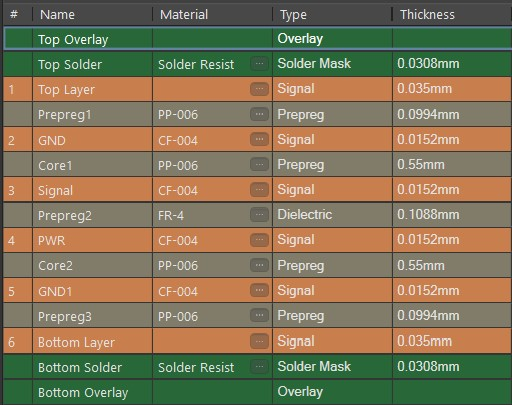
\includegraphics[scale=0.60]{PCB_mother_stackup.jpg}
		\caption{Rozložení vrstev PCB základní desky} 
		\label{fig:PCB_mother_stackup}
	\end{minipage}\hfill
	\begin{minipage}[b]{.45\linewidth}
		\centering
		\begin{tabular}{ |P{3cm}||P{3,5cm}|  }
			\hline
			\multicolumn{2}{|c|}{Rozložení vrstev PCB základní desky} \\
			\hline
			Vrstva  & Popis\\ \hline \hline 
			1 - TOP& Signálová vrstva\\ \hline		
			2 - GND1& Zemní vrstva \\ \hline 		 
			3 - SIG& Signálová vrsta \\ \hline
			4 - PWR& Napájecí vrstva\\ \hline
			5 - GND2& Zemní vrstva\\ \hline
			6 - BOT& Signálová vrstva\\ \hline
		\end{tabular}
		\caption{Popis vrstev PCB základní desky}
		\label{tab:pcb_vrstvy}
	\end{minipage}
\end{figure}

	\subsection{Napájení}
	Na základní desce je realizováno veškeré napájení, které je dále používáno pro celé výčítací rozhraní. Celkem jsou zde tři spínané synchronní step-down buck regulátory. Konkrétně se jedná o regulátor MP2333H \cite{MPH2333} od společnosti Monolithic Power Systems. Regulátor pracuje v rozsahu vstupních napětí on 4.2 - 18 V. Maximální výstupní proud jsou 3 A, spínací frekvence regulátoru je 1.2 MHz. Regulátor je možné pořídit v pouzdře SOT583, s rozměry 1.6x2 mm, které jsou pro úlohu minimalizace zařízení vyhovující. V tabulce \ref{tab:napajeni} můžete vidět seznam napájení dostupných na základní desce.
	\begin{table}[h!]
		\centering
		\begin{tabular}{ |P{3cm}||P{10cm}|  }
			\hline
			\multicolumn{2}{|c|}{Napájení základní desky vyčítacího rozhraní} \\
			\hline
			Napájení  & Popis\\ \hline \hline 
			+5V & Externí napájení vyčítacího rozhraní přes USB typu C. \\ \hline		
			+3V3 & Napájení pro mikrokontrolér, CPLD a další 3.3V periférie \\ \hline 		 
			+2V5 & Napájení vstupní a výstupní brány detektoru Timepix 2 \\ \hline
			+1V2 & Napájení jádra Timepix 2 a vstupní/výstupní brány CPLD.\\ \hline
		\end{tabular}
		\caption{Napájení základní desky vyčítacího rozhraní}
		\label{tab:napajeni}
	\end{table}
	Všechny napájení uvedené v tabulce \ref{tab:napajeni} jsou dostupné také na druhé desce plošných spojů, chipboardu. Více o propojení signálů základní desky a chipboardové desky lze dohledat v části \ref{konektor}. Ukázkové schematické zapojení jednoho ze tří spínaných regulátorů, můžete vidět na obrázku \ref{fig:mp2333h}. Konkrétně se jedná o zapojení, při kterém regulátor reguluje z +5 V napájení na napájení +1.2 V.
	\begin{figure}[h!]
		\centering
		\captionsetup{justification=centering}
		\includegraphics[scale=0.80]{mp2333h.jpg}
		\caption{Zapojení regulátoru MP2333H} 
		\label{fig:mp2333h}
	\end{figure}
	\subsubsection{Napájecí sekvence}
	Napájecí sekvenci je možné vidět na zjednodušeném diagramu na obrázku \ref{fig:napajeci_sekvecne}. Po připojení USB typu C do konektoru na základní dece je dostupné napájení +5 V. Těchto +5 V spíná první regulátor, který generuje na výstupu +3.3 V napájení. Pokud je toto výstupní napájení +3.3 V v pořádku, integrovaný obvod tuto informaci signalizuje pomocí pinu PG. Právě tento pin PG, signál PG\_3V3, je připojen na vstupní pin dalšího regulátoru a to na pin regulátoru generující výstupní napětí +2.5 V. Poslední regulátor s výstupním napětí +1.2 V je řízený z mikrokontroléru, jeho vstupní pin EN je propojen signálem EN\_1V2 s výstupní bránou mikrokontroléru.
	\begin{figure}[h!]
		\centering
		\captionsetup{justification=centering}
		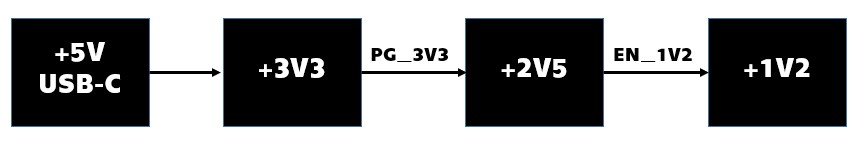
\includegraphics[scale=0.80]{napajeci_sekvence.jpg}
		\caption{Napájecí sekvence základní desky} 
		\label{fig:napajeci_sekvecne}
	\end{figure}
	\par Výstupní napětí spínaného regulátoru je nastaveno pomocí napěťového děliče ve zpětné vazbě regulátoru a dáno vztahem dle \ref{eq:Vout}. Kde $V_{REF}$ = 805 mV.
	\begin{equation}
		V_{OUT} = \frac{R1 \cdot V_{REF}}{R2} + V_{REF}
		\label{eq:Vout}
	\end{equation}

	\par Z obrázku \ref{fig:napajeci_sekvecne} je vidět, že spínaná stabilizátory pro +3.3 V a +2.5 V nejsou programově ovladatelné z mikrokontroléru. Spínaný stabilizátor +3.3 V, z mikrokontroléru řídit nelze, protože právě těchto +3.3 V je napájením pro vybraný mikrokontrolér. Možností jakým mimo jiné zajistit dodržení vhodného časování napájecí sekvence základní desky, je propojení PG signálu stabilizátoru +3.3 V na signál EN stabilizátoru +2.5 V. Další možností rozfázování napájecí sekvence je volba vhodného kondenzátoru mezi pinem SS a zemním pinem ze zapojení \ref{fig:mp2333h}. Kde $V_{REF}$ = 805 mV a $I_{SS}$ = 7.3 $\mu$A.
	\begin{equation}
		T_{SS}\,[ms] = \frac{2V_{REF} \cdot C_{SS} \,[nF]}{I_{SS}}
		\label{eq:Tss}
	\end{equation}
	Ze zapojení \ref{fig:mp2333h} a dosazení do vzorce \ref{eq:Tss} můžeme dopočítat, že rozběhový čas spínaného zdroje bude 1.4 ms. Ověření funkčnosti napájecí sekvence viz. \ref{fig:napajeci_sekvence_real}. Kde CH1 je napájení +1.2 V, CH2 je +2.5 V a CH3 je vstupních +5V. Na nastavených kurzorech je také vidět, že teoreticky vypočítaný čas, doby rozběhu regulátoru z rovnice \ref{eq:Tss}, souhlasí s prakticky naměřenými hodnoty. 
	\begin{figure}[h!]
		\centering
		\captionsetup{justification=centering}
		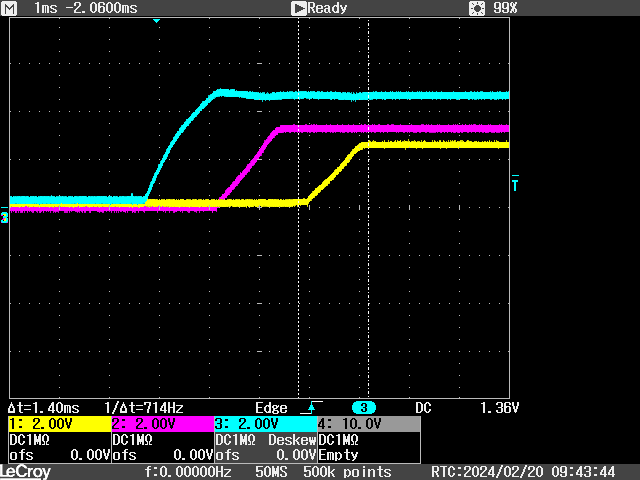
\includegraphics[scale=0.50]{napajeci_sekvence_real.png}
		\caption{Měření napájecí sekvence základní desky} 
		\label{fig:napajeci_sekvecne_real}
	\end{figure}
	
	\par Ochrana vstupního napájení bude popsána v části \ref{USB}. Pouze ve shrnutí, pokud dojde k jakýmkoliv podmínkám které by mohli elektricky ohrozit vyčítací rozhraní obvody z části \ref{USB} zajistí vypnutí napájení pomocí externího tranzistoru. 
	%TODO Dodat ??? spabilita napapájení

	\subsection{Mikrokontrolér}
	\label{mikrokontolér}
	Pro tuto práci byl vybrán mikrokontrolér od firmy STMicroelectronics, přesněji mikrokontrolér s označením STM32U5A9NJH6Q \cite{STM32U5A9}. Právě tento mikrokontrolér byl vybrán s ohledem na požadavky vyčítacího rozhraní, které byly uvedeny v předchozích částech textu. V následující části budou uvedeny nejdůležitější parametry vybraného mikrokontroléru:
	%\vspace{-5mm}
	\begin{itemize}
		\setlength\itemsep{0.005em}
		\item Jádro : Arm 32-bit Cortex-M33 s DSP a FPU. Frekvence 160 MHz
		\item Napájení 1.7 - 3.6 V
		\item Při provozu 18.5 $\mu$A/MHz
		\item 4-Mbyte flash s EEC
		\item 2514-Kbyte RAM, 66 Kbytes s EEC
		\item 25 Komunikačních periférií
		\item 156 konfigurovatelných vstupních/výstupních pinů
		\item 1 USB OTG high-speed s embedded PHY 
		\item Pouzdro : TFBGA216. 13 x 13 mm, 0.8 mm mezi pájecími plošky
	\end{itemize}
	\par Prvním požadavkem na mikrokontrolér bylo, aby bylo možné komunikovat přes sériovou datovou linku s detektorem Timepix 2. V již popsané části textu \ref{Komunikacni rozhrani}, bylo zmíněno, že Timepix 2, dokáže komunikovat po sériové lince s maximální frekvencí 100 Mhz. Výše uvedený vybraný mikrokontrolér umožňuje konfiguraci komunikačního kanálu, konkrétněji specfikace SPI až do frekvence 160 MHz. 
	\par Dalším důležitým parametrem při výběru mikrokontroléru byla velikost paměti. Pro vyčtení jedné matice pixelů z detektoru Timepix 2, z výše popsané části textu \ref{Digitálni cast} vyplývá, že je zapotřebí vyčíst 28x256x256 bitů dat, tedy 229.376 kB. Výše vybrané parametry pamětí mikrokontroléru jsou pro tento datový tok dostačující.
	\par Nejméně důležitým parametrem při výběru mikrokontroléru byl parametr integrovaného USB přímo uvnitř mikrokontroléru. Není tedy zapotřebí při návrhu USB umísťovat další součástky pro implementaci USB komunikace. Tímto parametrem mikrokontroléru dokážeme výrazně snížit počet použitých součástek a tím tak i rozměry celého vyčítacího rozhraní.
	
	\subsubsection{Konfigurace mikrokontroléru}
	Pro práci s mikrokontrolérem jsem použil vývojové prostředí STM32CubeIDE dodávané od společnosti STMicroelectronics, která je výrobcem vybraného mikrokontroléru. Výhodou vývojového prostředí je přímočará grafická konfigurace celého mikrokontroléru. Na obrázku \ref{fig:STM32CubeIde} můžete vidět příklad nakonfigurovaného mikrokotroléru STM32U5A9 v pouzdře TFBGA216. Tmavě zelené body mezi piny znamenají uživatelsky nastavené rozhraní daného pinů mikrokontroléru.
	
	\subsubsection{Napájení}
	Na obrázku \ref{fig:napajeni_stm32} můžete vidět potřebná napájení pro vybraný mikrokontrolér. Více podrobností ohledně napájení lze najít v referenčním manuálu viz. \cite{STM32U5A9_RM}. Realizace shematického zapojení napájení mikrokontroléru viz přiložená příloha. %TODO odkaz na prilohu
	\begin{figure}[h!]
		\begin{subfigure}{0.5\textwidth}
			\centering
			\captionsetup{justification=centering}
			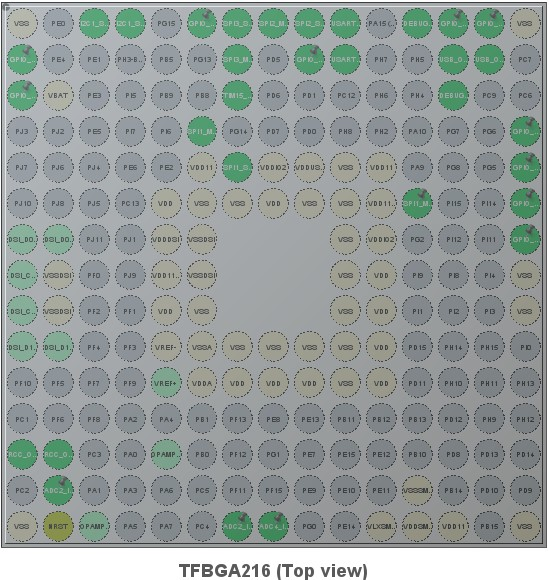
\includegraphics[scale=0.60]{STM32CubeIde.jpg}
			\caption{STM32CubeIDE konfigurace pinů mikrokontroléru} 
			\label{fig:STM32CubeIde}
		\end{subfigure}
		\begin{subfigure}{0.5\textwidth}
				\centering
			\captionsetup{justification=centering}
			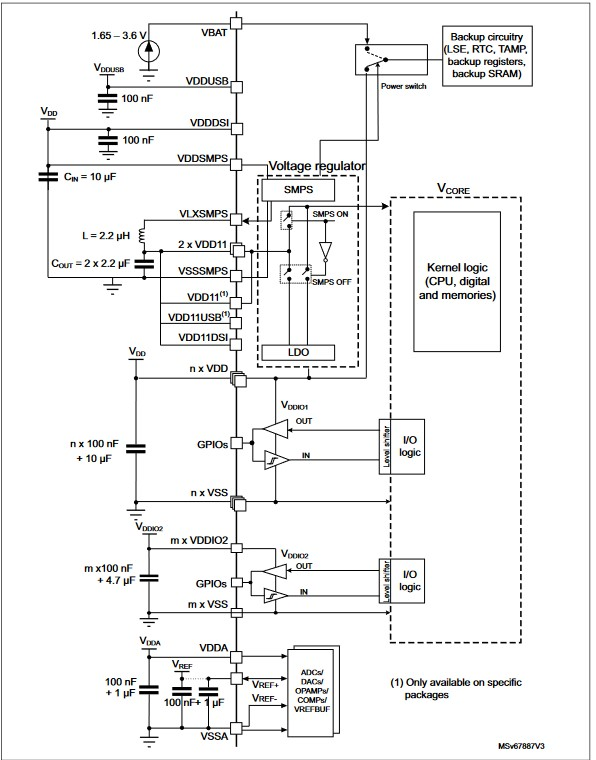
\includegraphics[scale=0.60]{STM32_napajeni.jpg}
			\caption{STM32U5A9 napájení} 
			\label{fig:napajeni_stm32}
		\end{subfigure}
		\caption{Konfigurace a napájení STM32U5A9}
		\label{fig:konfig}
	\end{figure} 
	\begin{table}[h!]
		\centering
		\begin{tabular}{ |P{3cm}||P{10cm}|  }
			\hline
			\multicolumn{2}{|c|}{Napájení základní desky vyčítacího rozhraní} \\
			\hline
			Napájení  & Popis\\ \hline \hline 
			VBAT & Napájení z externí baterie 1.65 - 3.6 V\\ \hline		
			VDDUSB & Napájení periférie USB\\ \hline 		 
			VDDSI & Napájení pro periféri DSI \\ \hline
			VDDSMPS & Napájení pro integrovaný spínaný stabilizátor\\ \hline
			VLXSMPS & Spínaný výstup integrovaného stabilizátoru \\ \hline
			VDD11 & Napájení digitální části mikrokotroléru \\ \hline 
			VDD11, VDD & Napájení digitální části mikrokotroléru ze spínaného stab.\\ \hline
			VDDIO2 & Napájení samostatné vstupní/výstupní brány \\ \hline
			VDDA & Napájení analogové části mikrokotroléru \\ \hline
		\end{tabular}
		\caption{Napájení mikrokontroléru STM32U5A9}
		\label{tab:napajeni_stm32}
	\end{table}
	Výhodou vybraného mikrokontroléru je, že pro napájení jádra a digitálních periferií využívá spínaného regulátoru integrovaného přímo na čipu, který má nižší spotřebu oproti lineárnímu regulátoru. Nevýhodou tohoto napájení je požadavek připojení externí cívky, která je nezbytná pro provoz interního spínaného stabilizátoru a tím tak větší požadavky na rozměry celého zapojení. 
	\subsubsection{Konfigurace hodinových signálů} %Pro USB HS plus konfigurace ostatnich periferii ?
	Hodinový signál (SYSCLK) pro jádro mikrokontroléru může být vybrán jeden ze čtyř dostupných zdrojů hodinového signálu, kterými jsou:
	\begin{itemize}
		\setlength\itemsep{0.005em}
		\item HSE : Externí krystal s parametry frekvencí hodin od 4 MHz do 50 Mhz
		\item HSI : 16 MHz interní RC oscilátor 
		\item MSI : Interní RC oscilátor s programově nastavitelnou frekvencí od 100 kHz do 48 MHz
		\item PLL : Fázový závěs, který může mít vstup jeden ze 3 výše uvedených zdrojů hodinového signálu
	\end{itemize}
	Pro realizaci vyčítacího rohraní byl jako zdroj hodinového signálu vzbrán výstup fázového závěsu, který ze vstupního hodinového signálu HSI generuje hodinový signál o frekvenci 160 MHz. Tento hodinový signál je použit jako zdroj hodinového signálu pro jádro mikrokontroléru a také pro komunikační rozhraní, až na komunikační rozhraní USB. Více o popisu konfigurace hodinového signálu pro USB periferii viz část textu \ref{USB}. Konfiguraci hodinového signálu (SYSCLK) pro jádro procesoru s využitím fázového závěsu, lze najít na obrázku \ref{fig:hodinovy_signal} 
	\begin{figure}[h!]
		\centering
		\captionsetup{justification=centering}
		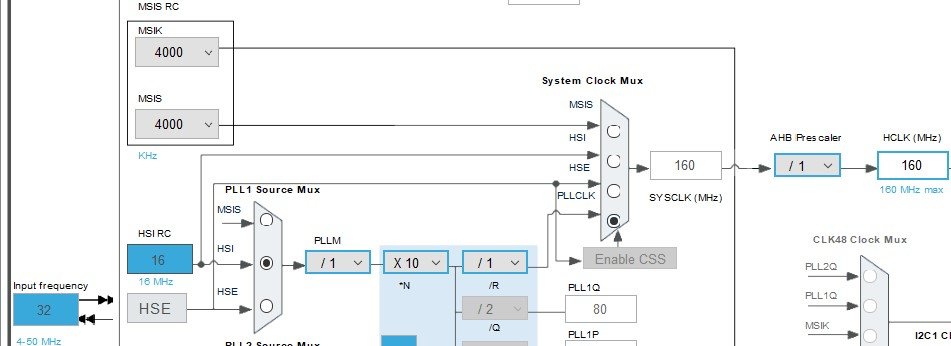
\includegraphics[scale=0.65]{hodinovy_signal.jpg}
		\caption{Konfigurace hodinového signálu pro jádro mikrokontroléru} 
		\label{fig:hodinovy_signal}
	\end{figure}

	\subsubsection{Konfigurace komunikačních sběrnic}
	Celkem pro implementaci vyčítacího rozhraní byly použity tři SPI periférie:
	 \begin{itemize}
	 	\setlength\itemsep{0.005em}
	 	\item SPI1 : Použito jako obecné SPI pro komunikaci se senzory, mimo Timepix 2
	 	\item SPI2 : Slouží ke komunikaci s Timepix 2. Konfigurace master. 
	 	\item SPI3 : Slouží ke komunikaci s Timepix 2  Konfigurace slave.
	 \end{itemize}
 	Sběrnice SPI1 je nakonfigurována v modu Full-Duplex Master. K určení jaké zařízení budou komunikovat po sběrnici slouží signály chip select (nCS), prefix n, značí, že signál je aktivní v logické nule. Pro komunikaci s Timepix 2 byly svoleny dvě periférie SPI. SPI1 je nakonfigurována jako master. Tedy pomocí této sběrnice se odesílají data do detektoru Timepix 2. SP2 je nakonfigurována jako typ slave, tedy pomocí této sběrnice se příjmají data z detektoru Timepix 2.
 	
 	\par Další sběrnicí používané vyčítacím rozhraním je sběrnice I2C. Pro celé rozhraní byla použita právě jedna I2C periférie. Pomocí této sběrnice mikrokotrolér monitoruje teplotu na druhé desce plošného spoje, chipboardu. Více o komunikaci s teplotním senzorem viz. \ref{Mereni teploty}.
 	
 	\par Dále byla nakonfigurována periférie UART, tato periférie umožňuje monitorovat průběh firmwaru za použití výpisu do příkazové řádky. Signály UART sběrnice jsou vyvedeny na programovací konektor, jak bylo popsáno výše.

%TODO zminit literaturu ZAHLAVA A MCU
	\subsubsection{Programování}
	Mikrokontrolér je programován pomocí JTAG rozhraní za využití programovacího konektoru, který je umístěn na spodní straně desky, viz obrázek \ref{fig:programator}. Jedná se o 12 pinový konektor pro plochý kabel. Pro programování mikrokontroléru byly konkrétně vyvedeny signály: JTMS/SWDIO a JTCK/SWCLK. Zbylé piny konektoru byly využity pro programování MachXO2 \cite{CPLD}. Tedy přes plochý konektor z obrázku \ref{fig:programator} lze progrmovat jak mikrokontolér, tak na základní dece použité CPLD: MachXO2 \ref{CPLD}. Posledními signály vyvedenými na programovací konektor jsou signály pro monitorování běhu programu, jedná se o signály komunikačního rozhraní sběrnice UART. Signály jsou za pomocího plochého kabelu vyvedeny z plochého konektrou z obrázku \ref{fig:programator} na redukční desku, na které je možné pomocí propojovacích kabelů připojit použitý programátor ST-Link, právě s navrženou konverzní deskou. Toto jednoduché PCB můžete vidět na obrázku \ref{fig:konverzni_deska}. 
\begin{figure}[h!]
	\begin{subfigure}{0.5\textwidth}
		\centering
		\captionsetup{justification=centering}
		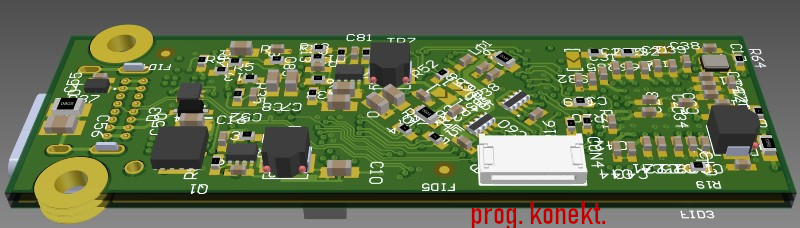
\includegraphics[scale=0.50]{programator.jpg}
		\caption{Programovací konektor} 
		\label{fig:programator}
	\end{subfigure}
	\begin{subfigure}{0.5\textwidth}
		\centering
		\captionsetup{justification=centering}
		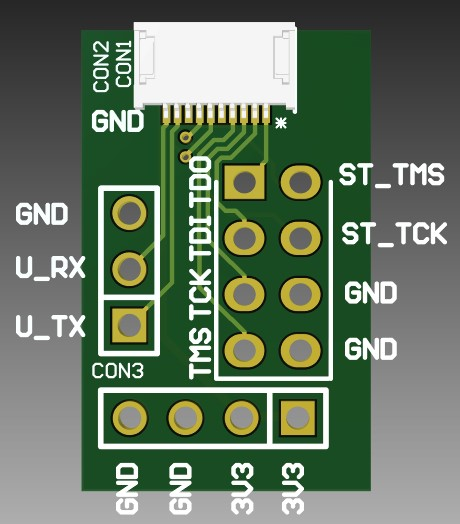
\includegraphics[scale=0.30]{konverzni_deska.jpg}
		\caption{Konverzní PCB pro připojení ST-Link programátoru} 
		\label{fig:konverzni_deska}
	\end{subfigure}
	\caption{Programování mikrokontroléru}
	\label{fig:programovani}
\end{figure} 

	\subsubsection{PCB}
	Realizované PCB pro část mikrokontroléru můžete vidět na obrázku \ref{fig:ST_layout}. Na obrázku nejsou uvedeny 3 zbylé vrstvy PCB, kterými jsou 2., 3. a 5. vrstva. Vrstva 2 a 5 tvoří pod částí mikrokontroléru souvislou zemní plochu a vrstva 3 slouží jako vrstva signálová. Blokovací kondenzátory napájení dle specifikací \cite{STM32U5A9_RM} jsou umístěny co nejblíže příslušným pinům, z druhé strany, než je samotná mikrokontrolér, viz. \ref{fig:ST_BOT}. 
	\begin{figure}[h!]
		\centering
		\captionsetup{justification=centering}
		\begin{subfigure}[b]{0.3\textwidth}
			\centering
			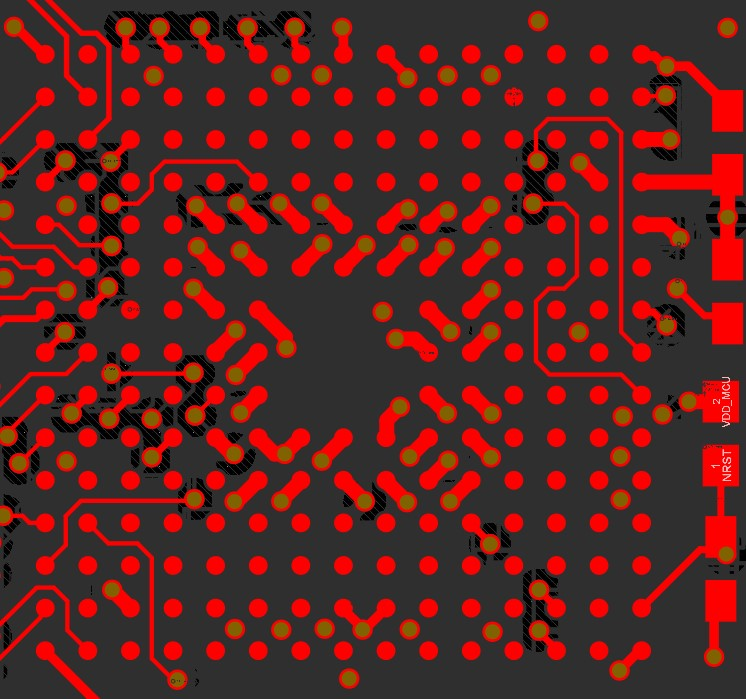
\includegraphics[scale=0.30]{ST_TOP.jpg}
			\caption{Vrchní vrstva PCB STM32U5A9}
			\label{fig:ST_TOP}
		\end{subfigure}
		\hfill
		\begin{subfigure}[b]{0.3\textwidth}
			\centering
				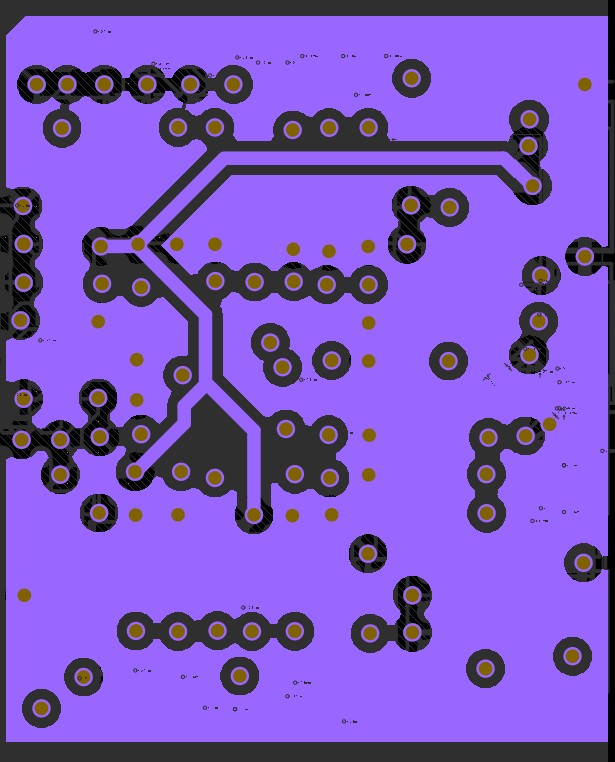
\includegraphics[scale=0.30]{ST_PWR.jpg}
			\caption{Prostřední vrstva PCB STM32U5A9}
			\label{fig:ST_PWR}
		\end{subfigure}
		\hfill
		\begin{subfigure}[b]{0.3\textwidth}
			\centering
				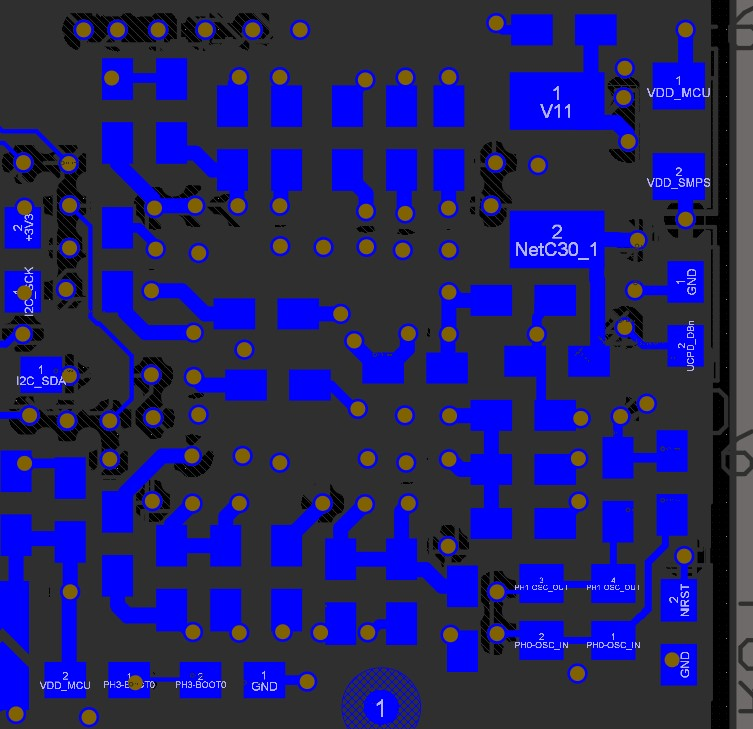
\includegraphics[scale=0.30]{ST_BOT.jpg}
			\caption{Spodní vrstva pcb STM32U5A9}
			\label{fig:ST_BOT}
		\end{subfigure}
		\caption{STM32U5A9 PCB realizace}
		\label{fig:ST_layout}
	\end{figure}
	Rozteč mezi jednotlivými piny mikrokontroléru je 0.8 mm. Jak lze vidět na obrázku \ref{fig:ST_TOP}, mezi pájecími plošky jsou umístěny prokovy. Vnitřní průměr prokovů je 0.3 mm a vnější rozměr 0.4 mm. Prokovy jsou kvůli zvolenému pouzdru mikrokontroléru (BGA) zamaskované, aby při procesu pájení nedošlo ke zkratování prokovů s piny mikrokontroléru.
	\par Osazení mikrokontroléru proběhlo na půdě ČVUT v laboratoři LVR (Laboratoř pro Vývoj a Realizaci). Pro osazení byl použita rework stanice: ERSA - IRPL650A.
	
	\subsection{CPLD}	% CPLDcko - delice, urovne. Odporove site
	\label{CPLD}
	\subsubsection{Konverze logických úrovní}
	Dle \ref{kap:3.2.1}, je zapotřebí při komunikaci s Timepix 2 po sériové sběrnici použít diferenciální páry, konkrétněji použít komunikační specifikaci SLVS. Použití mikrokontrolér \ref{mikrokontolér}, je kompatibilní pouze s CMOS 3.3V logikou. Pro převod 
	\subsection{USB} % Navrh plosnaku, USB C ochrana, popis USB C konektoru
	\label{USB}

%TODO kde popisu cely cyklus vycitani? v Testovani?
% TODO cite zahlava
\section{Deska s Timepix 2}
	\subsection{Timepix 2}	% 
		\subsubsection{Rozhraní pro připojení Timepix 2}	% wirebondovaci plosky, HV zdroj
		\subsubsection{Napájení}	% popsat jak se bere z konektoru plus prepinani pro chipID
	\subsection{Vysokonapěťový zdroj}	% MAX1932 zapojeni vysvetleni
		\subsubsection{Měření vysokého napětí} % napetovy sledovac plus konfigurace AD v STM32
	\subsection{Měření teploty}	% proces nastaveni senzoru atd
	\label{Mereni teploty}
	\subsection{Konektor}	% popis konektoru, zarazeni zmneni mezi piny
	\label{konektor}


\chapter{Testování}
%TODO vysledky zobrozene v TrackLabu !

%TODO mozna neco z testovani zaradit do sekce realizace. predevsim nejake promerovani parametru? a tady nechat jen zasadni info o dulezitych testech
\section{Napájení}
% TODO V2 uvest rozbehove sekvence celeho zarizeni  !!
% TODO V2 stailita 1V2ANA 1V2DIG pro Timepix2 !!
Na základní desce jsou generované celkem 3 napájecí úrovně z +5V externího napájení přes USB, jak bylo uvedeno v sekci \ref{napajeni}. A to napájecí úrovně +1.2 V, +2.5 V a +3.3 V. Zvlnění výstupního napětí bylo poté vždy měřeno na výstupu každého spínaného regulátoru se snahou vytvoření co nejkratší zemní smyčky mezi měřícím bodem a připojenou zemí osciloskopu. Měření nebylo ve všech případech s ohledem na velikost zemní smyčky ideální vzhledem k zapojení ve kterém je realizováno vyčítací rozhraní a to tedy v zapojení, kdy je deska s Timepix 2 nad základí deskou a tedy není možné se připojit sondou osciloskopu na vrchní stranu základní desky. I s ohledem na zmíněné problémy byly naměřeny tyto průběhy \ref{fig:napeti}. Kde CH3 je +2.5 V, CH2 +3.3V a CH1 poté +1.2 V.
\begin{figure}[h!]
	\centering
	\captionsetup{justification=centering}
	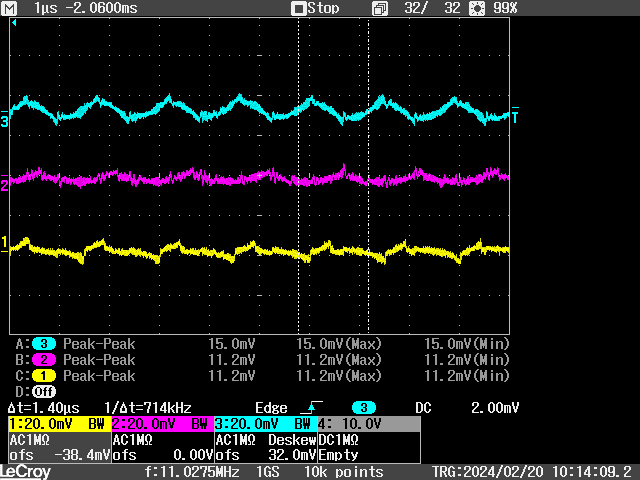
\includegraphics[scale=0.40]{./Mereni/ripple 3V3 - CH2 & 2V5 - CH3 & 1V2 - CH1, 2x 47uF.png}
	\caption{Zvlnění napětí výstupních napětí +2.5V, +3.3 V a +1.2 V } 
	\label{fig:napeti}
\end{figure}
Stabilní stejnosměrné hodnoty výše uvedených napájecích úrovní je možné vidět na obrázku 
\begin{figure}[h!]
	\centering
	\captionsetup{justification=centering}
	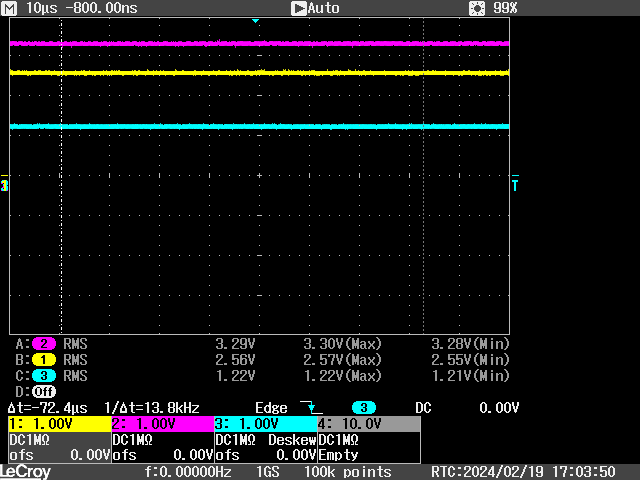
\includegraphics[scale=0.40]{./Mereni/vout 3V3 & 2V5 & 1V2.png}
	\caption{Stjenosměrné úrovně výstupních napětí spínaných regulátorů na základní desce \ref{zakladni deska}} 
	\label{fig:urovne}
\end{figure}

%todo ripple output of HV?
\section{Vysokonapěťový zdroj}
% Nastaveni VN zdroje
Zapojení vyskonapěťového zdroje a princip měření vysokého napětí, které se generuje na desce s Timepix 2 \ref{Deska s Timepix2} je popsán v části textu \ref{VN zdroj}. Velikost vysokého napětí je nastavována pomocí 8 bitového čísla. Závislost 8 bitové hodnoty na výstupním napětí vysokonapěťového zdroje je možné vidět na obrázku \ref{fig:hv_hex}.
\begin{figure}[h!]
	\centering
	\captionsetup{justification=centering}
	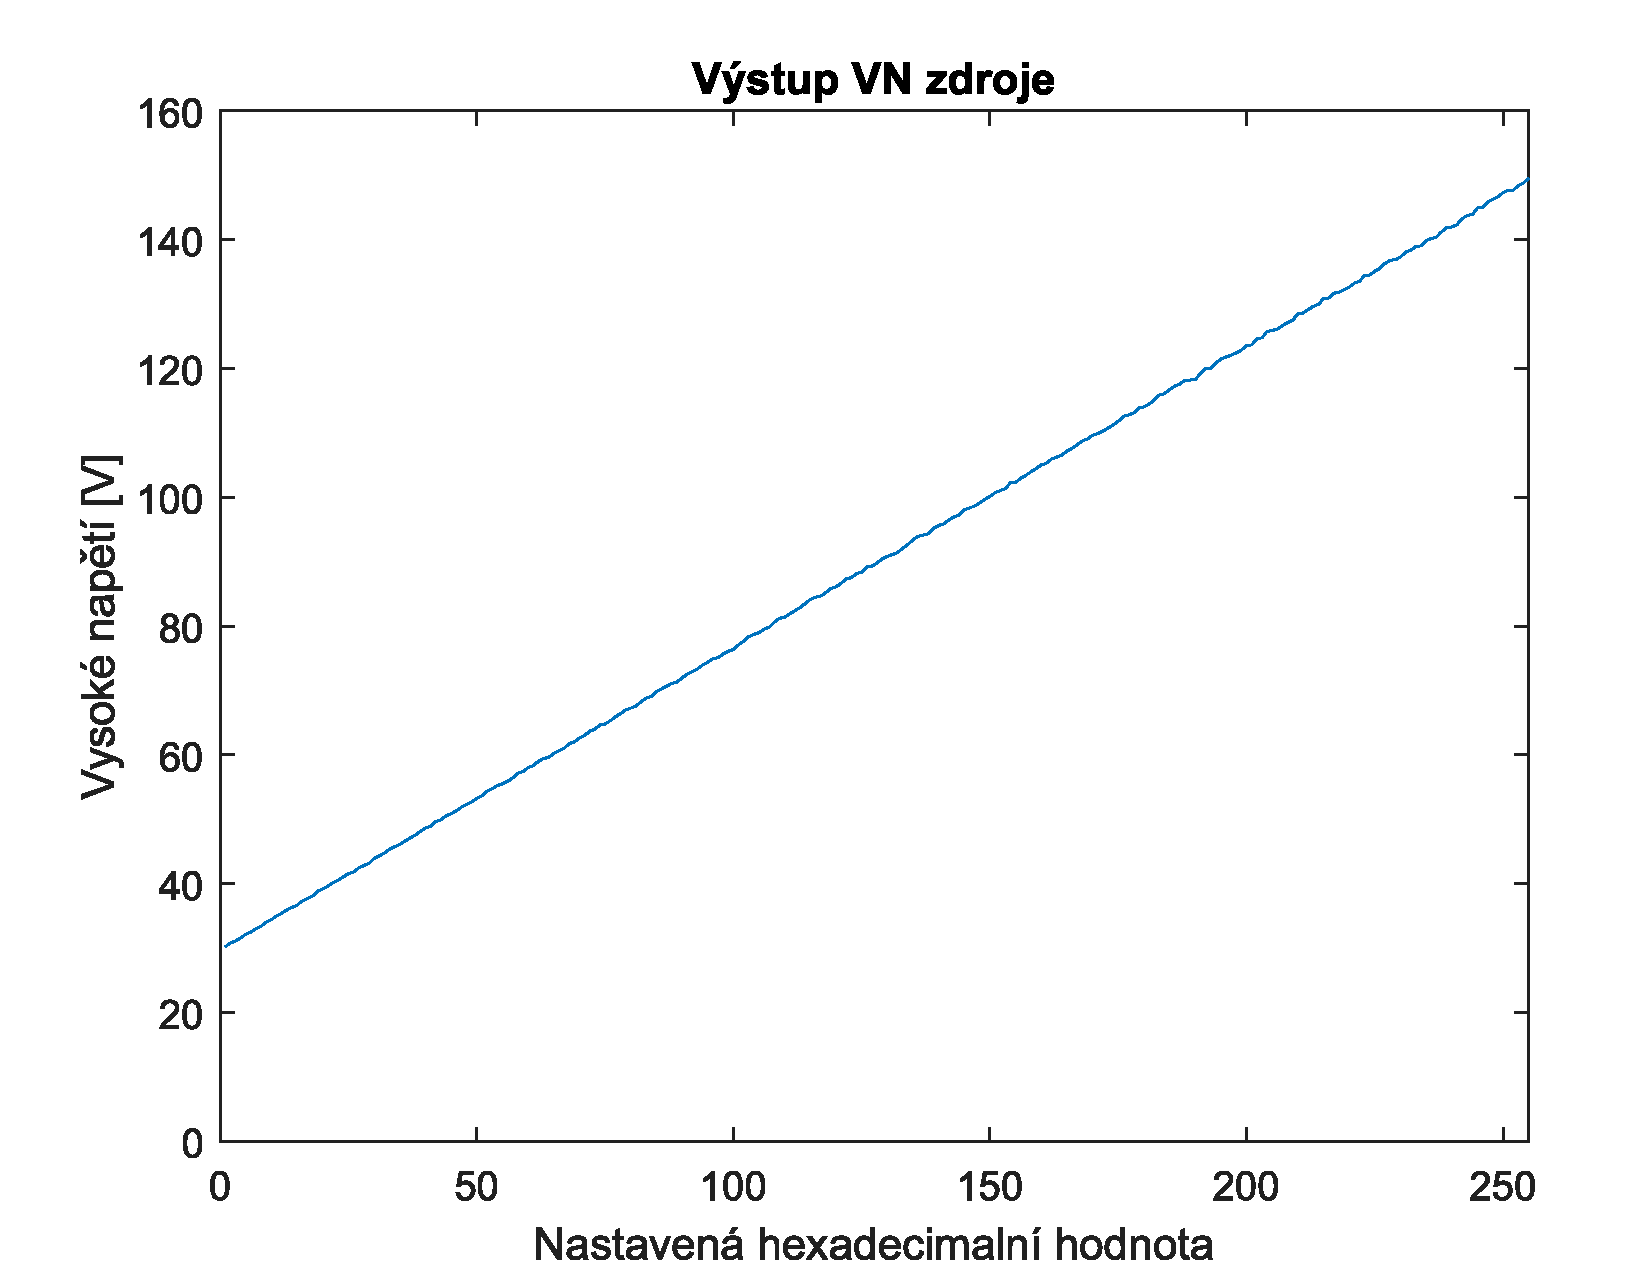
\includegraphics[scale=0.40]{./Mereni/hv_hex_small.pdf}
	\caption{Závislost vstupní 8 bitové hodnoty na výstupním napětí VN zdroje} 
	\label{fig:hv_hex}
\end{figure}
 
\section{Měření teploty}
V této práci bylo implementováno měření teploty pomocí externího teplotního senzoru na desce s detektorem Timepix 2 \ref{Deska s Timepix2} a měření teploty za využití interního měření teploty detektoru Timepix 2.
% TODO výpis z Terminalu, jeste lepe z TrackLabu
% TODO promereni teploty s mechanikou ??
\subsection{Měření teploty vyčítacího rozhraní}
Typ senzoru který byl pro tuto práci vybrán pro měření teploty na desce s Timepix 2 byl podrobně popsán v části \ref{Mereni teploty}. Pokud dojde k uživatelskému příkazu, který požaduje informaci o teplotě, následuje proces vyčtení teploty ze senzoru, který je zjednodušeně popsán diagramem na obrázku \ref{fig:diagram}.
\begin{figure}[h!]
	\centering
	\captionsetup{justification=centering}
	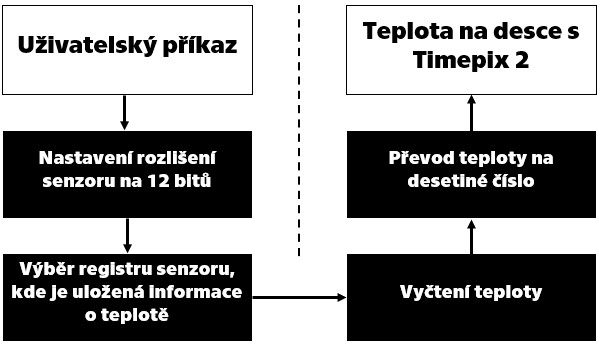
\includegraphics[scale=0.50]{teplota diagram.jpg}
	\caption{Diagram průběhu vyčtení teploty ze senzoru TMP 100 na desce s Timepix 2} 
	\label{fig:diagram}
\end{figure}

\subsection{Měření teploty Timepix2}
Pixelový detektor Timepix 2 umožnuje monitorovat vnitřní teplotu detektoru. Hodnota výsledné teploty detektoru je poté dle simulace teploty detektoru v závislosti na napěťové referenci popsána na obrázku \ref{fig:tpx2_temp}. Pro získání teploty detektoru je zapotřebí naměření dvou analogových hodnot z obrázku \ref{fig:tpx2_temp} označovaných jako Vtemp a Vbg. Pro získání těchto analogových hodnot je nejprve zapotřebí nastavit, jaká hodnota analogového napětí bude na výstupu pinu Timepix 2 označovaného jako DACOUT. Výstup DACOUT Timepix 2 je poté zpracován interním ADC převodníkem mikroprocesoru na základní desce \ref{zakladni deska}. Příklad výběru hodnoty na výstup DACOUT detektoru Timepix 2 a převod získaných hodnot na odpovídající teplotu lze vidět v \ref{kod_temp_tpx2}.
\begin{lstlisting}[frame=single, language=C, caption={Výběr výstupu DACOUT detektoru Timepix2 a odečtení hodnoty detektoru}, label=kod_temp_tpx2]
// GET DAC : VBG_TEMP
uint8_t set_dacoutsel[0] = VBG_TEMP; 
float vtemp = 0;
// set what type of DAC will be on DACOUT output								   
if(tpx2_set_reg_8b(TPXA, SET_DACOUTSEL, set_dacoutsel) != TPX_OK) {    
	Error_Handler();
}
if(board_tpx2_get_dacout(TPXA, &vtemp) != BOARD_OK) {
	Error_Handler();
}
// Sim. -> TT. // Temp. into real value in ^C.
float tpx2_temp = 471.99*(vtemp - vbg)/1000 - 179.14;					
\end{lstlisting}

\begin{figure}[h!]
	\centering
	\captionsetup{justification=centering}
	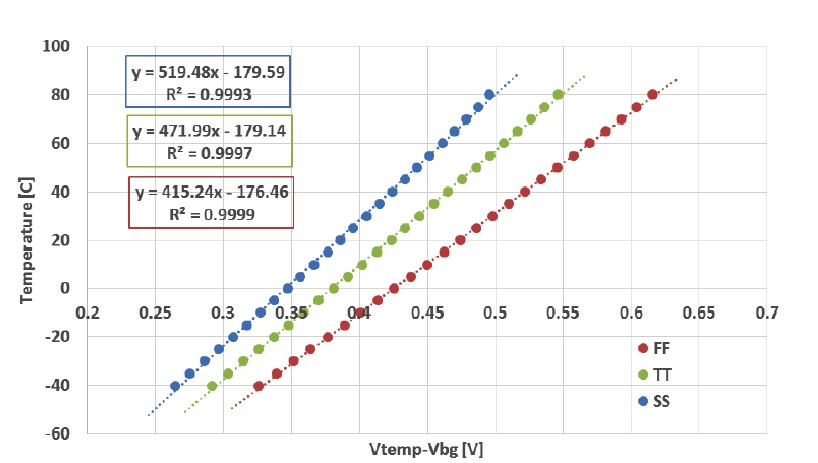
\includegraphics[scale=0.50]{tpx2_temp.jpg}
	\caption{Simulace teploty detektoru Timepix2 v závisloti na hodnotě napěťové reference \cite{tpx2_manual}.} 
	\label{fig:tpx2_temp}
\end{figure}



\section{Komunikační rozhraní s Timepix 2}		% promřování logických urovni komunkikace, rychlosti atd..
%todo logicke urovne SLVS, rychlosti komunikace -> need V2. MCLOCK..
Komunikační rozhraní detektoru Timepix 2 bylo popsáno v části textu \ref{Komunikacni rozhrani}. Následná  realizace komunikace s Timepix 2 pak v části \ref{CPLD konverze}. K měření diferenciálních komunikačních signálů byla použita aktivní diferenciální sonda s osciloskopem. Měření probíhalo při frekvenci komunikace 20 Mhz. Na obrázku \ref{fig:MCLOCK_DIFF_PROBE} můžete vidět průběh komunikačních hodin. Konkrétně CH 2 z obrázku \ref{fig:MCLOCK_DIFF_PROBE} je výstup hodinového signálu SPI komunikace. Kanál CH 1 je poté naměřený diferenciální signál aktivní diferenciální sondou po konverzi logické úrovně v CPLD. Jak je vidět parametry diferenciálního signálu odpovídají parametrů SLVS komunikace. 
\begin{figure}[h!]
	\centering
	\captionsetup{justification=centering}
	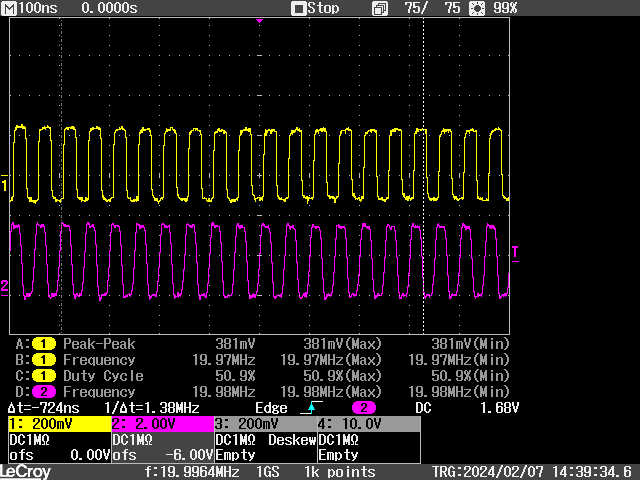
\includegraphics[scale=0.40]{./Mereni/MCLOCK_DIFF_PROBE.png}
	\caption{Průběh hodinového signálu pro komunikaci s Timepix 2} 
	\label{fig:MCLOCK_DIFF_PROBE}
\end{figure}

\section{Digitální test Timepix 2} %popis prubehu a vysledku
Funkčnost komunikace s detektorem Timepix 2 byla ověřena pomocí digitálních testů, jednotlivé testy budou popsány v následujících částech.
	\subsection{Vyčtení chip ID}
	Prvním digtálním testem, který byl implementován byl test, který vyčítá sériové výrobní číslo, označované jako CHIP ID, které je pro každý detektor Timepix 2 jedinečné a předem známé. Pro správné vyčtení CHIP ID detektoru je nejprve zapotřebí přivést napájecí napětí +2.5 V na pin VDD33, jak bylo popsáno v části \ref{Technicka specifikace}. Hodnota CHIP ID je poté uložena v 32-bitové registru Timepix 2. Vyčtením tohoto registru dostáváme 32 bitovou hodnotu, kterou pomocí známé transformace převedeme na skutečnou hodnotu CHIP ID, která odpovídá předem známé hodnotě, jež je dodávaná přímo při dodání detektoru Timepix 2.
	%TODO hodnota CHIP ID
	\subsection{Vyčtení a zapsání pixelových matic}
	Pomocí výše uvedeného testu, vyčtení CHIP ID detektoru došlo k otestování vyčítaní základních registrů detektoru Timepix 2. Dalším digitálním testem je poté zápis a vyčtení všech čítačů, používajících se na měření. Popis čítačů Timepix 2, lze najít v části \ref{Digitálni cast}.
	\par Zápis do digitálních čítačů slouží jen pro digitální testování, při samotném měření se tato funkce nevyužívá. Celkem při tomto digitálním testu dochází k zápisu hodnot do všech čtyřech dostupných čítačů Timepix 2 a následnému vyčtení. Celkem je zapsáno 5 testujících obrazů. Zapsané obrazce byly zvoleny viz. tabulka \ref{tab:obraz}. Při tomto digitálním testu dochází k zápisu 327 680B dat a jejich opětovnému vyčtení. Digitální test byl prováděn s frekvencí datových hodin 40 Mhz. Po každém digitálním testu bylo vyresetováno napájení detektoru Timepix 2 a digitální test byl proveden znovu. Test byl opakován 100 krát s úspěšností 100\%.
	\begin{table}[h!]
		\centering
		\begin{tabular}{ |P{3cm}|P{3cm}|  }
			\hline
			\multicolumn{2}{|c|}{Vybrané zapsané obrazce} \\
			\hline
			Test  & Obraz\\ \hline \hline 
			1 & 0xFF \\ \hline 	
			2 & 0x00 \\ \hline 		 
			3 & INC \\ \hline
			4 & DEC \\ \hline
			5 & 0xAA\\ \hline
		\end{tabular}
		\caption{Digitální test, zapisované hodnoty}
		\label{tab:obraz}
	\end{table}
\section{USB komunikace}
%todo, dokumentace funkčnosti... -> VCM, pak UDP pres USB
Fyzická implementace USB byla popsána v části textu \ref{USB}. Pro testování USB komunikace byly použity dvě USB třídy. První třídou USB byl virtuální sériový port přes USB. Druhou USB třídou byla pak třída RNDIS, neboli virtuální ethernet přes USB.
\subsection{Virtuální sériový port}
	První třídou testující funkčnost USB byl virtuální sériový port. Tato třída byla na začátek vybrána díky své jednoduchosti. Nakonfigurované USB zařízení, tedy vyčítací rozhraní z této práce, připojené do PC s operačním systémem Windows 10 můžete vidět na obrázku \ref{fig:USB_VCM}. Tato konfigurace sloužila pouze pro první ověření funkcionality USB rozhraní.
	%TODO vypis ze seriaku/USBTreeViewer
	\begin{figure}[h!]
		\centering
		\captionsetup{justification=centering}
		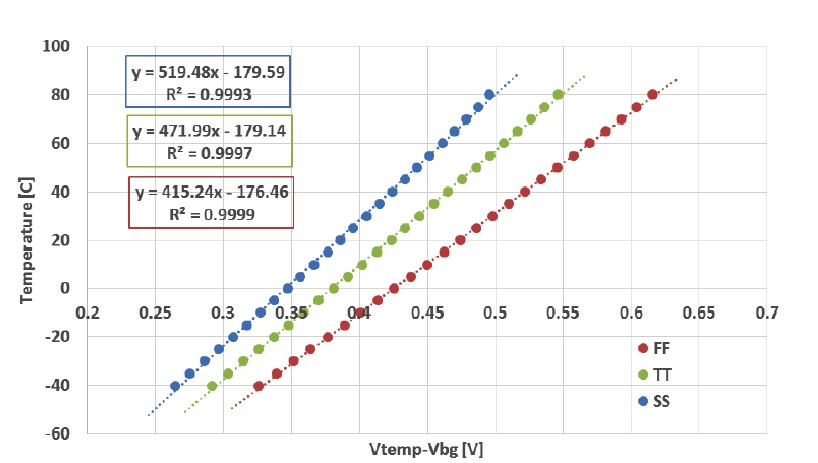
\includegraphics[scale=0.50]{tpx2_temp.jpg}
		\caption{Výpis virtuální sériové komunikace přes USB} 
		\label{fig:USB_VCM}
	\end{figure}
\subsection{Virtuální ethernet přes USB}
	Další USB třídou, která se již použila v konečné implementaci byla USB třída RNDIS. Jedná se o třídu zařízení kdy je přes USB implementován virtuální ethernet. V této práci se konkrétně pomocí USB přenáší UDP komunikace. Tato třída byla zvolena s ohledem na existující program TrackLab \cite{TrackLab}. TrackLab umožňuje připojit různá vyčítací rozhraní s pixelovými detektory. Vyčítací rozhraní v této práci respektuje již existující standart a to standart připojení vyčítacího rozhraní Katherine pro Timepix 2 \ref{Katherine}. Ukázka nakonfigurovaného zařízení jako třída RNDIS lze vidět na obrázku \ref{fig:RNDIS}.
	%TODO USB RNDIS konfigurace
	\begin{figure}[h!]
		\centering
		\captionsetup{justification=centering}
		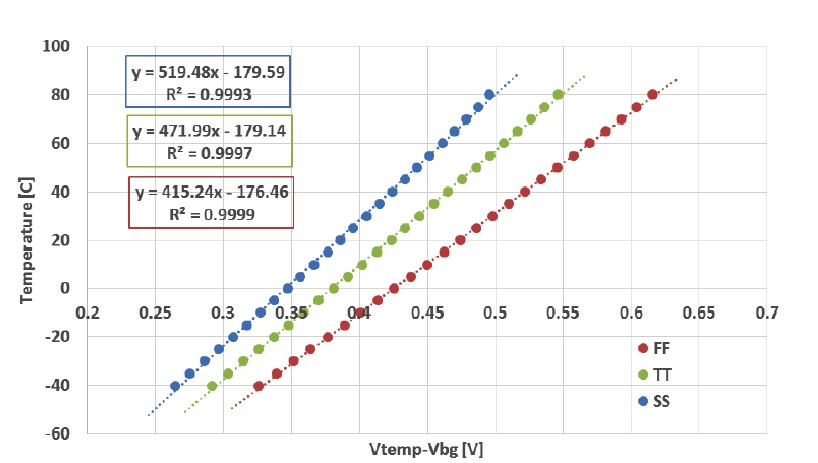
\includegraphics[scale=0.50]{tpx2_temp.jpg}
		\caption{Vyčítací rozhraní nakonfigurované jako zařízení z USB třídy RNDIS} 
		\label{fig:RNDIS}
	\end{figure}
%TODO mam dat zvlast tridu o TrackLabu?
	

\section{Měření spotřeby}
%todo spotreba, bez chipu, s chipem, zavislosti?
	\subsection{Porovnání spotřeby} % TODO nebo jen uvest parametry?
	
\section{Dosažené parametry}
% TODO shrnuti nosazenych parametru namerenych vyse

\chapter{Závěr}

V této práci bylo navrženo miniaturizované vyčítací rozhraní pro pixelový detektor radiace Timepix 2. Tato práce probíhala na půdě Ústavu Technické a Experimentální fyziky ČVUT v Praze. 

Vyčítací rozhraní se skládá ze dvou desek plošných spojů, které jsou vertikálně propojeny pomocí konektoru. Jedná se o základní desku a desku s detektorem Timepix 2. Jádrem základní desky je mikroprocesor STM32 v pouzdře BGA, který se používá k ovládání celého rozhraní. Na druhé desce plošných spojů se nachází detektor Timepix 2, který slouží k sofistikovanému měření ionizujícího záření. Tento detektor je propojen wire bondovací technologií s deskou plošných spojů. Spotřeba navrženého rozhraní, pokud je plně v provozu je 1.5 W. Celé vyčítací rozhraní je poté zapouzdřeno mechanickou hliníkovou krabičkou o rozměrech 73.4 x 22 x 13.5 mm.

Dále bylo realizováno propojení navrženého rozhraní s již existujícím programem TrackLab \cite{Manek_2024}, který slouží pro zpracování dat z pixelových detektorů, online analýzu a automatizaci. Toto propojení je realizováno pomocí virtuálního ethernetu přes USB s maximální teoretickou přenosovou rychlostí 480 Mbit/s.
 
Funkčními testy byla ověřena funkčnost rozhraní, kdy hlavní testem bylo reálné měření s navrženým vyčítacím rozhraním na urychlovači částic v laboratoři CERN. Měřeny byly částice o energii 10 GeV. Rychlost vyčítaní dat z detektoru Timepix 2 byla nastavena na 40 Mbit/s. Z analýzy naměřených dat a průběhu celého měření byla potvrzena schopnost používat navržené rozhraní pro reálné měření ionizujícího záření. 
\newline
\par
Výsledkem této práce je navržené miniaturizované vyčítací rozhraní pro pixelový detektor radiace Timepix 2, které je možné používat pro sofistikované fyzikální experimenty měřící ionizující záření. Díky propojení rozhraní do programu TrackLab je možné naměřená data živě zobrazovat, vyhodnocovat a celé měření automatizovat. 



%literatura
\renewcommand{\bibname}{Seznam použité literatury}
\bibliography{references}
\bibliographystyle{ieeetr}
\addcontentsline{toc}{chapter}{Seznam použité literatury}

% TODO edit zkratky
\chapwithtoc{Seznam použitých symbolů}
\begin{tabular}{ l  l }
	
	$\alpha$ 			& alfa 				\\
	
\end{tabular}

\chapwithtoc{Seznam použitých zkratek}
\begin{tabular}{ l  l }
	
	ASIC & Application Specify Integrated Circuit \\
	TSMC & Taiwan Semiconductor Manufacturing Company Limited \\ 
	TSV	 & Through-Silicon-Vias \\
	BGA & Ball Grid Array \\
	FPGA & Field Programmable Gate Arrays \\
	CMOS & Complementary metal–oxide–semiconductor \\
	DAC & Digital to Analog Convertor \\
	LSFR & Linear Feedback Shift Registers \\
	PCB & Printed Circuit Board \\
	HV & High Voltage \\
	USB & Universal Serial Bus \\
	DSP & Digital signal processing \\
	FPU & Floating Point Unit \\
	EEC & Error Correction Code \\
	ESD & Electro Static Discharge \\
	DSI & Display Serial Interface \\
	PG & Power Good \\
	EN & Enable \\
	SYSCLK & System Clock \\
	HSI & High Speed Internal Clock \\
	HSE & High Speed Internal Clock \\
	PLL & Phase Locked Loop \\
	JTAG & Joint Test Action Group \\
	CPLD & Complex Programmable Logic Devices \\
	SPI & Serial Peripheral Interface \\
	UART & Universal Asynchronous Receiver-Transmitter \\
	ZCS & Zero Column Suppression \\
	SYSCLK & System Clock \\
	
	
		
\end{tabular}
% TODO include zadnání diplomky plus prilohy (viz. BP)
\appendix

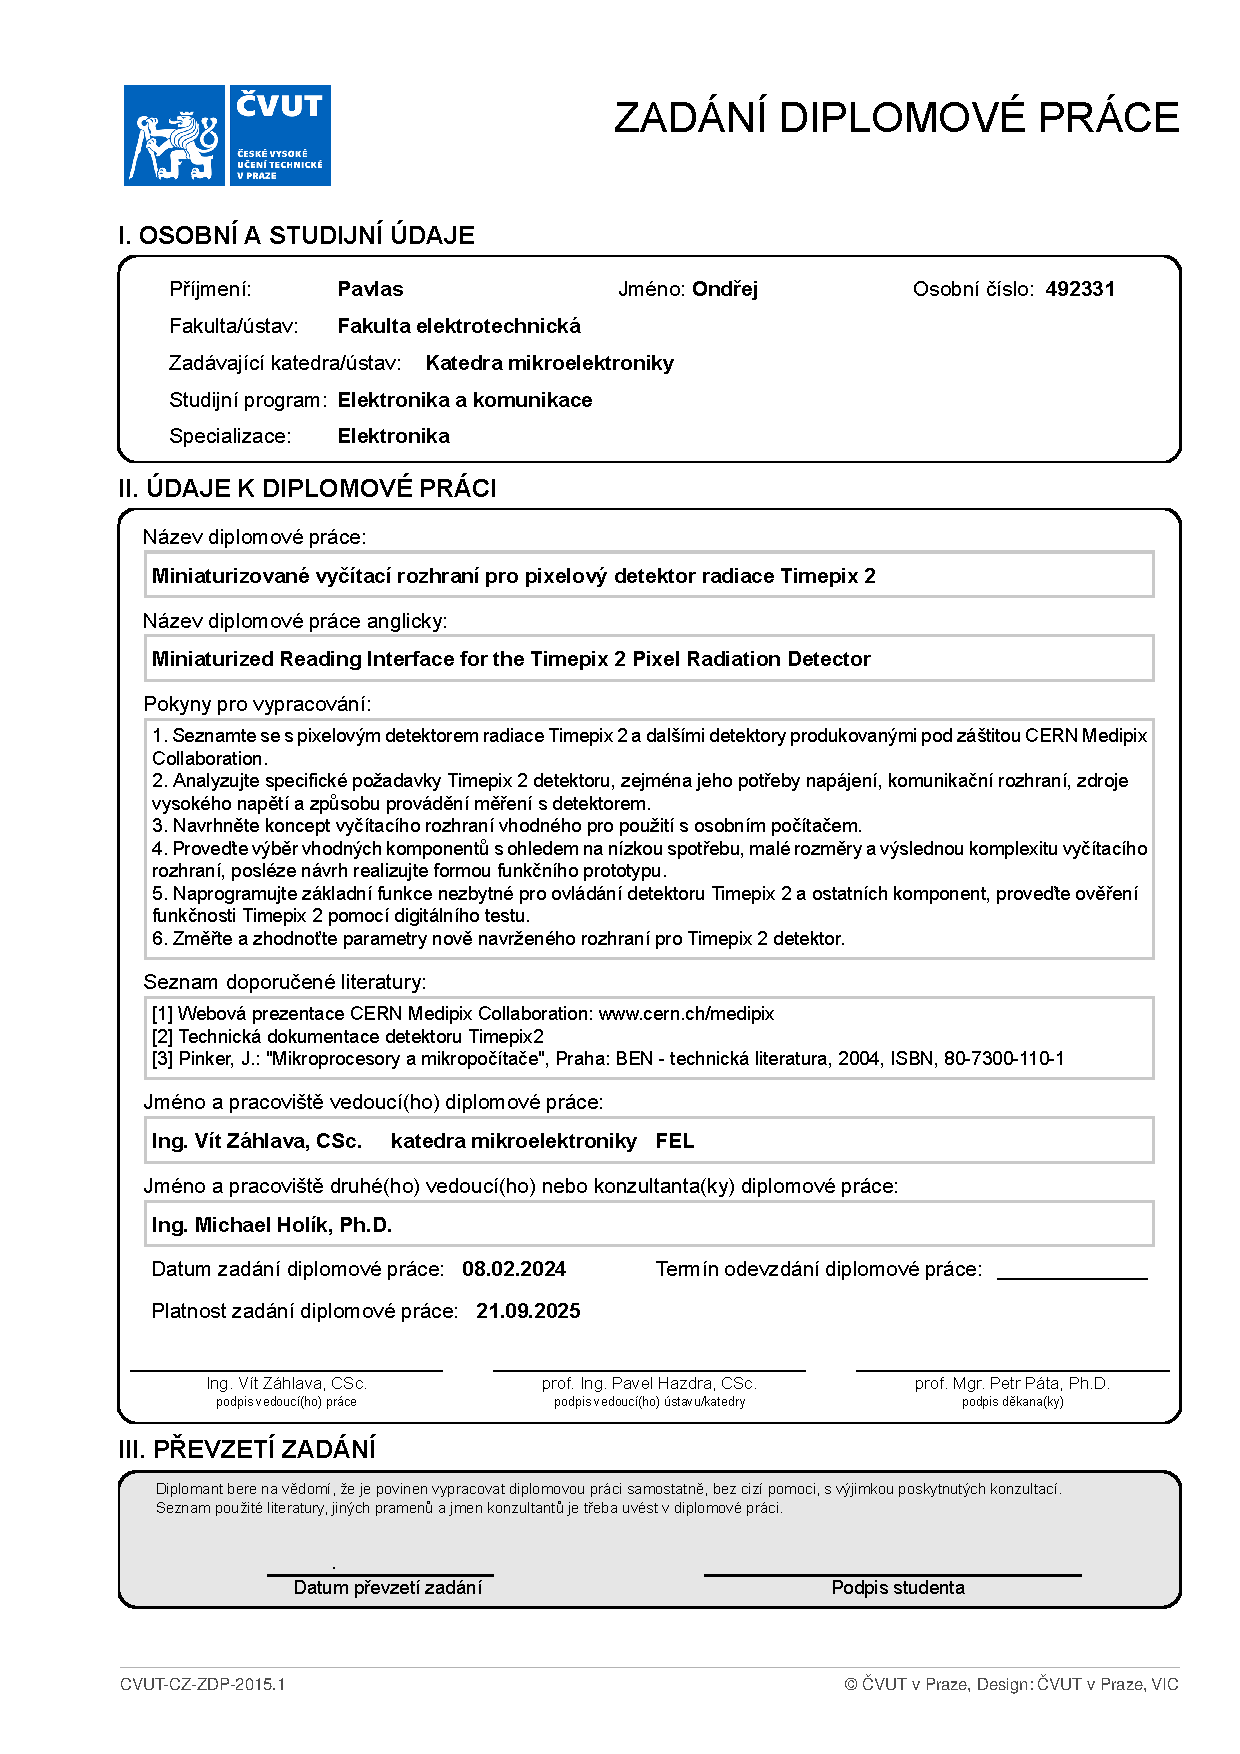
\includepdf[scale=0.7, offset=20 -80,pages=1,pagecommand=\chapter{Zadání Diplomové práce}]{./zadani.pdf}
\chapter{Základní deska}
\label{Priloha základní deska}

	
\end{document}




